\documentclass{wccm2024}

\usepackage{graphicx}
\usepackage{amsmath}
\usepackage{amsfonts}
\usepackage{amssymb}
\usepackage{times}
\usepackage{xcolor}
\usepackage{subfig}
\usepackage{stmaryrd}

\title{A primal hybrid finite element method to solve general compressible, quasi-incompressible and incompressible elasticity using stable H(div)-L2 spaces}

\author{PHILIPPE R. B. DEVLOO$^{1}$, GIOVANE AVANCINI$^{2}$, NATHAN SHAUER$^{3}$ AND HUGO L. OLIVEIRA$^{4}$}

\heading{Philippe R. B. Devloo, Giovane Avancini, Nathan Shauer and Hugo Luiz Oliveira}

\address{$^{1}$ State University of Campinas, Faculty of Civil Engineering\\
Av. Albert Einstein, 901 - Cidade Universitária, Campinas - SP, 13083-852\\
phil@unicamp.br
\and
$^{2}$ State University of Campinas, Faculty of Civil Engineering\\
Av. Albert Einstein, 901 - Cidade Universitária, Campinas - SP, 13083-852\\
giovanea@unicamp.br
\and
$^{3}$ State University of Campinas, Faculty of Civil Engineering\\
Av. Albert Einstein, 901 - Cidade Universitária, Campinas - SP, 13083-852\\
shauer@unicamp.br
\and
$^{4}$ State University of Campinas, Faculty of Civil Engineering\\
Av. Albert Einstein, 901 - Cidade Universitária, Campinas - SP, 13083-852\\
hluiz@unicamp.br}

\keywords{Hybrid finite element method, incompressible elasticity, De Rham compatible spaces}

\abstract{Hybrid methods are usually derived from an extended variational principle, in which the interelement continuity of the functions subspace is removed and weakly enforced by means of a Lagrange multiplier. In this context, a new primal hybrid finite element formulation is presented, which uses H(div) conforming displacement functions and discontinuos L2 approximation for pressure together with shear traction functions to weakly enforce tangential displacement. This combination allows the simulation of compressible, quasi-incompressible and fully incompressible elastic solids, with convergence rates independent of its bulk modulus. The proposed approach benefits from the property that the divergence of the H(div) displacement functions is De Rham compatible with the (dual) pressure functions. The hybridization of the tangential displacements is weakly enforced through a lower order shear stress space. This leads to a saddle-point problem that is stable over the full range of poisson coefficient (large compressibility up to incompressible). Moreover, a boundary stress (normal and shear) can be recovered that satisfies elementwise equilibrium. Hybridizing the tangent stresses and condensing the internal degrees of freedom, a positive-definite matrix with improved spectral properties can be recovered. The stability, consistency and local conservation features are discussed in details. The formulation is tested and verified for different test cases.}

\begin{document}
\thispagestyle{empty}

\section{INTRODUCTION}

In the context of linear elasticity, several numerical methods have been developed in the past years. The most used one is the Finite Element Method (FEM). Using a continuous Galerkin approach to approximate the displacements may lead to shear-locking phenomenon due to spurious energy modes under bending \cite{bletzinger2000unified,belytschko1985stress} or volume-locking under quasi or full incompressibility, as the stresses go to infinity \cite{neto2005f,cervera2003mixed}.

There are different ways in the literature to overcome these drawbacks. One possible choice is to employ a mixed formulation \cite{brezzi2012mixed,arnold1988new} where the displacements and the stresses (or pressure) are approximated independently - i.e. the Taylor Hood elements \cite{taylor1973numerical} fulfill the \textit{inf-sup} condition yielding stable results for incompressible regime. This kind of approximation, on the other hand, is not locally conservative as it does not satisfy the divergence constraint in a strong manner. Another possibility is to use hybrid methods where the interelement continuity of a given field is broken and weakly imposed by means of a Lagrange multiplier (see for instance \cite{raviart1977primal,harder2016hybrid,farhloul1997dual}).

In this work we extend the semi-hybrid approach proposed in \cite{carvalho2024semi} for Stokes problems to develop a new primal hybrid finite element formulation for elasticity based on a De Rham compatible pair $H(\text{div})-L^2$ for normal displacements and pressure. The $H(\text{div})$ functions are constructed using a systematic methodology described in \cite{devloo2022efficient,de2013new}.

\section{GOVERNING EQUATIONS}

In general elasticity, the governing equation of a continuum body $\Omega \in \mathbb{R}^3$ is given by:
\vskip-.3cm
\begin{equation} \label{eq:strong1}
    -\nabla \cdot \boldsymbol{\sigma} - \mathbf{b} = \mathbf{0} \hspace{0.2cm} \text{in } \Omega \text{,} 
\end{equation}

\noindent where $\boldsymbol{\sigma}$ denotes the Cauchy stress tensor and $\mathbf{b}$ is the body forces vector. For the well-posedness sake, proper boundary conditions need to be imposed on the Dirichlet boundary ($\partial\Omega_D$) and on the Neumann boundary ($\partial\Omega_N$), as said,
\vskip-.3cm
\begin{equation}
    \mathbf{u} = \mathbf{u}_D \hspace{0.2cm} \text{on } \partial\Omega_D \text{,}
\end{equation}
\vskip-.3cm
\begin{equation}
    \boldsymbol{\sigma} \cdot \mathbf{n} = \mathbf{h} \hspace{0.2cm} \text{on } \partial\Omega_N \text{.} 
\end{equation}

The Generalized Hook law relates the stresses and strains by:
\vskip-.3cm
\begin{equation}
    \boldsymbol{\sigma} = 2\mu \boldsymbol{\varepsilon} + \lambda \text{tr}(\boldsymbol{\varepsilon}) \mathbf{I} \text{,}
\end{equation}

\noindent where $\mu$ and $\lambda$ are known as Lamé constants, $\boldsymbol{\varepsilon}$ is the infinitesimal strain tensor, computed as:
\vskip-.3cm
\begin{equation} \label{eq:strain}
    \boldsymbol{\varepsilon}=\frac{1}{2}(\nabla\mathbf{u}^T+\nabla\mathbf{u}) \text{,}
\end{equation}

\noindent and $\mathbf{I}$ is the identity matrix. By recalling that the hydrostatic pressure is defined as

\begin{equation}
    p = -\frac{\text{tr}(\boldsymbol{\sigma})}{3}=-\frac{(2\mu+\lambda)}{3}\text{tr}(\boldsymbol{\varepsilon}),
\end{equation}

\noindent and considering that $\boldsymbol{\sigma} = \boldsymbol{\sigma}'-p\mathbf{I}$, Eq. \eqref{eq:strong1} can be rewritten in a mixed form so the boundary-valued problem reads:
\vskip-.3cm
\begin{equation} \label{eq:strong2}
    \begin{cases}
        -\nabla \cdot \boldsymbol{\sigma}'\left(\mathbf{u}\right) + \nabla p - \mathbf{b} = \mathbf{0} \hspace{0.2cm} \text{in } \Omega\\
        -\nabla \cdot \mathbf{u} - \frac{1}{\kappa}p = 0\hspace{0.2cm} \text{in } \Omega\\
        \mathbf{u} = \mathbf{u}_D \hspace{0.2cm} \text{on } \partial\Omega_D\\
        \boldsymbol{\sigma} \cdot \mathbf{n} = \mathbf{h} \hspace{0.2cm} \text{on } \partial\Omega_N
    \end{cases}
\end{equation}

\noindent where $\kappa=\frac{2\mu+\lambda}{3}$ is the material bulk modulus, $\mathcal{D}^{'}$ is the fourth-order deviatoric part of the elasticity tensor and $\boldsymbol{\sigma}'$ refers to the deviatoric stress, computed as:
\vskip-.3cm
\begin{equation}
    \boldsymbol{\sigma}' = 2\mu \left(\boldsymbol{\varepsilon} - \frac{1}{3}\text{tr}(\boldsymbol{\varepsilon})\right) \text{.}
\end{equation}

One notices that when $\lambda \rightarrow \infty$, Eq. \eqref{eq:strong2} recovers the classical mass conservation form of an incompressible material i.e. $\nabla \cdot \mathbf{u}=0$.

\section{WEAK FORM AND FINITE ELEMENT DISCRETIZATION}

The variational form of Eqs. \eqref{eq:strong2} can be obtained by means of the weighted residual method. Depending on the choice of test functions and approximation spaces, different formulations can be derived. We shall start from the most simplistic one, the primal displacement formulation and then move to the double-hybrid scheme.

Let $\mathcal{T}=\{\Omega_e,e=1, \cdots, n_e \}$ be a partition of $\Omega$ in $n_e$ finite elements $\Omega_e$ with hexahedral shape for $d=3$. The set $\mathcal{E}$ contains all the element edges $E$ and $\mathcal{E}_0=\{E \in \mathcal{E} : E \subset \Omega \}$ denotes the internal edges or element interfaces. Let introduce the following function spaces: 

\subsection{Primal displacement formulation}

The primal displacement formulation is obtained by multiplying Eq. \eqref{eq:strong1} by test functions $\mathbf{v} \in \mathbf{V}\text{ } | \text{ }\mathbf{V} \subset H^1(\mathcal{T})$ and integrating over the discretized domain $\mathcal{T}$ \cite{becker1981finite}. The weak statement reads: find $\mathbf{u} \in \mathbf{V}$ such that for all $\mathbf{v} \in \mathbf{V}$,

\begin{equation} \label{eq:primal-displacement}
    \sum_{\Omega_e \in \mathcal{T}} \int_{\Omega_e} \boldsymbol{\varepsilon}(\mathbf{u}) : \mathcal{D}^{'} : \boldsymbol{\varepsilon}(\mathbf{v}) d\Omega_e = \sum_{\Omega_e \in \mathcal{T}} \left(\int_{\Omega_e} \mathbf{b} \cdot \mathbf{v} d\Omega_e + \int_{\Gamma_N} \mathbf{h} \cdot \mathbf{v} d\partial\Omega_e \right)
\end{equation}

\noindent is satisfied. Although the primal displacement formulation is simple to implement, it has some limitations i.e. locking phenomena under bending and incompressibility. To overcome these limitations, we shall introduce the semi-hybrid formulation.

\subsection{Mixed formulation}
The mixed formulation is obtained by multiplying the first equation in Eq. \eqref{eq:strong2} by test functions $\mathbf{v} \in \mathbf{V}\text{ } | \text{ }\mathbf{V} \subset H^1(\mathcal{T})$ and by multiplying the second equation in Eq. \eqref{eq:strong2} by $q\in L^2(\Omega)$ and integrating over the discretized domain $\mathcal{T}$. The weak statement reads: find $\mathbf{u} \in \mathbf{V}$ and $p\in L^2(\Omega)$ such that for all $\mathbf{v} \in \mathbf{V}$ and $q\in L^2(\Omega)$,

\begin{equation} \label{eq:mixedA}
        \int_{\Omega} \boldsymbol{\varepsilon}(\mathbf{v}) : \mathcal{D}^{''} : \boldsymbol{\varepsilon}(\mathbf{u}) d\Omega - \int_{\Omega_e} p \;(\nabla \cdot \mathbf{v}) d\Omega =  \int_{\Omega} \mathbf{v} \cdot \mathbf{f} d\Omega + \int_{\Gamma} \mathbf{v} \cdot \boldsymbol{\sigma}_N d\partial\Omega
\end{equation}
\begin{equation} \label{eq:mixedB}
    -\int_{\Omega} (\nabla \cdot \mathbf{u}) \;q\; d\Omega -\int_{\Omega} \frac{3}{2\mu+\lambda}\;p \;q\; d\Omega = \mathbf{0}
\end{equation}

\subsection{Semi-hybrid formulation}

In \cite{carvalho2024semi}, the authors proposed a semi-hybrid formulation for Stokes-Brinkman flows that uses $H(\text{div})$ conforming velocity functions and discontinuos $L^2$ approximation for pressure. The same ideia can also be applied to elasticity. Let $\mathcal{V} = \mathbf{V}\cap H(\text{div},\Omega)$, $\Psi \subset L^2(\Omega)$ be spaces of vector functions and piece-wise scalars, respectively, for which the relation $\nabla \cdot \mathcal{V} \in \Psi$ holds. As $H(\text{div})$ approximation only guarantees the continuity of normal componentes of a vector across elements interface, a hybridization of the tangential velocity is performed. We introduce a third space defined as $\boldsymbol{\Lambda}^t \subset H^{-1/2}(\partial\Omega_e)$, for which the Lagrange multiplier $\boldsymbol{\lambda}^t \in \boldsymbol{\Lambda}^t$ has the meaning of a shear traction to weakly enforce the tangential displacement continuity. 

The weak statement for the semi-hybrid formulation thus reads: find $\{\mathbf{u},p,\boldsymbol{\lambda}^t\} \in \mathcal{V} \times \Psi \times \boldsymbol{\Lambda}^t$ such that for all $\{\mathbf{v},q,\boldsymbol{\eta}^t\} \in \mathcal{V}\times \Psi \times \boldsymbol{\Lambda}^t$:

\begin{equation} \label{eq:semihybrid1}
    \begin{split}
        \sum_{\Omega_e \in \mathcal{T}} \left( \int_{\Omega_e} \boldsymbol{\varepsilon}(\mathbf{v}) : \mathcal{D}^{''} : \boldsymbol{\varepsilon}(\mathbf{u}) d\Omega_e - \int_{\Omega_e} p\; (\nabla \cdot \mathbf{v}) d\Omega_e \right) + \int_{\mathcal{E}^0} \boldsymbol{\lambda}^t \cdot \llbracket \mathbf{v} \rrbracket \;d\mathcal{E}^0 = \\ \sum_{\Omega_e \in \mathcal{T}} \left( \int_{\Omega_e} \mathbf{v} \cdot \mathbf{f} d\Omega_e + \int_{\Gamma} \mathbf{v} \cdot \boldsymbol{\sigma}_N \; d\partial\Omega_e \right)
    \end{split}
\end{equation}
\begin{equation} \label{eq:semihybrid2}
    \sum_{\Omega_e \in \mathcal{T}} \left(-\int_{\Omega_e} (\nabla \cdot \mathbf{u}) \;q\; d\Omega_e -\int_{\Omega_e} \frac{3}{2\mu+\lambda}\;p\; q\; d\Omega_e \right) = \mathbf{0}
\end{equation}
\begin{equation} \label{eq:semihybrid3}
    \int_{\mathcal{E}^0} \llbracket \mathbf{u} \rrbracket \cdot \mathbf{\eta}^t \;d\mathcal{E}^0 = \mathbf{0} \text{,}
\end{equation}

\noindent where $\mathbf{v}$, $q$ and $\boldsymbol{\eta}^t$ are test functions for velocity, pressure and tangential traction, respectively, $\llbracket \cdot \rrbracket$ stands for the jump operator on the interface $\mathcal{E}^0$ between two neighbour elements $\Omega_1$ and $\Omega_2$, defined as $\llbracket \mathbf{v} \rrbracket = \mathbf{v} \vert_{\Omega_1} - \mathbf{v} \vert_{\Omega_2}$. Equation \eqref{eq:semihybrid3} plays the role of weakly enforcing the tangential displacement continuity over the element interfaces.

\subsection{Double-hybrid formulation}

Although mathematically consistent, the semi-hybrid formulation poses some challenges from a numerical perspective. It gives rise to a saddle-point problem with two different constraints: $p$ and $\boldsymbol{\lambda}^t$. This structure significantly increases the efforts required to consistently and stably solve the linear system.

We propose a second hybridization of the tangential stresses in order to recover its primal form. Introducing the space $\mathcal{L}^t \subset H^{1/2}(\partial\Omega_e)$ for the tangential velocity, the hybrid form thus reads: find $\{\mathbf{u},p,\boldsymbol{\lambda}^t_e,\mathbf{u}^t\} \in \mathcal{V} \times \Psi \times \boldsymbol{\Lambda}^t \times \mathcal{L}^t$ such that for all $\{\mathbf{v},q,\boldsymbol{\eta}^t_e,\mathbf{v}^t\} \in \mathcal{V} \times \Psi \times \boldsymbol{\Lambda}^t\times \mathcal{L}^t$, the following equations are satisfied:

\begin{equation} \label{eq:hybrid1}
    \begin{split}
        \sum_{\Omega_e \in \mathcal{T}} \left( \int_{\Omega_e} \boldsymbol{\varepsilon}(\mathbf{v}) : \mathcal{D}^{''} : \boldsymbol{\varepsilon}(\mathbf{u})\; d\Omega_e + \int_{\Omega_e} p \;(\nabla \cdot \mathbf{v}) d\Omega_e - \int_{\partial\Omega_e} \boldsymbol{\lambda}^t_e \cdot \mathbf{v}\; d\partial\Omega_e \right) = \\ \sum_{\Omega_e \in \mathcal{T}} \left( \int_{\Omega_e} \mathbf{v} \cdot \mathbf{f} \;d\Omega_e + \int_{\Gamma} \mathbf{v} \cdot \boldsymbol{\sigma}_N\; d\partial\Omega_e \right)
    \end{split}
\end{equation}
\begin{equation} \label{eq:hybrid2}
    \sum_{\Omega_e \in \mathcal{T}} \left(-\int_{\Omega_e} (\nabla \cdot \mathbf{u})\; q \;d\Omega_e -\int_{\Omega_e} \frac{3}{2\mu+\lambda}\;p \;q \;d\Omega_e \right) = \mathbf{0}
\end{equation}
\begin{equation} \label{eq:hybrid3}
    \sum_{\Omega_e \in \mathcal{T}} \left(\int_{\partial\Omega_e} (\mathbf{u}^t-\mathbf{u}) \cdot \boldsymbol{\eta}^t_e\; d\partial\Omega_e \right)  = \mathbf{0}
\end{equation}
\begin{equation} \label{eq:hybrid4}
     \int_{\mathcal{E}^0} \left\langle \boldsymbol{\lambda}^t_e \right\rangle \cdot \mathbf{v}^t\; d\mathcal{E}^0 = \mathbf{0} \text{,}
\end{equation}

\noindent where Eq. \eqref{eq:hybrid4} was introduced to impose the continuity of the tangential traction across $\mathcal{E}^0$. Even though an additional constraint is introduced, $\boldsymbol{\lambda}^t$ is now associated to a single element therefore it can be statically condensed and eliminated from the global system. For a compressible solid, a symmetric positive-definite matrix is obtained with two unknowns, namely $\mathbf{u} \in H(\text{div},\Omega)$ and $\mathbf{u}^t \in H^{1/2}(\partial\Omega_e)$. For the incompressible case where pressures cannot be computed explicitly from the displacements, one mean pressure per element acts as a Lagrange multiplier in the global system. This still gives rise to a saddle-point matrix, however, with much better spectral properties and easier to solve compared to Eqs. \eqref{eq:semihybrid1}-\eqref{eq:semihybrid3}.

\section{NUMERICAL EXAMPLES}

This Section presents two examples to verify the primal hybrid formulation. The first one is a cantilever beam subjected to an end shear load, where a convergence test is carried out and compared to the analytical solution. The second example is a practical application where the proposed method was used to simulate a real structural casket used to run experimental analysis on petroleum engineering.

\subsection{Cantilever beam subjected to an end shear load \label{subsec:bishop}}

Figure \ref{fig:bishop-beam-geometry} shows a cantilever beam where $L=5$, $a=0.5$ and $b=0.5$. The beam is assumed to be fixed at $z=0$ and subjected to an unitary shear-force $F=\int_{-b}^{b}\int_{-a}^{a}\sigma_{yz}dxdy=1$ at $z=L$. The Young modulus is $E=1$ and different values for the poisson coefficient is used to test the formulation in different compressibility regimes, i.e. $\nu=0.3$, $\nu=0.4999$ and $\nu=0.5$.

\begin{figure}[!htb]
	\centering
	\subfloat[\label{fig:bishop-beam-geometry}]{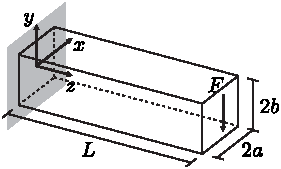
\includegraphics[scale=1.0]{figs/bishop-beam-geometry.pdf}} \hfill
    \subfloat[\label{fig:bishop-meshes-a}]{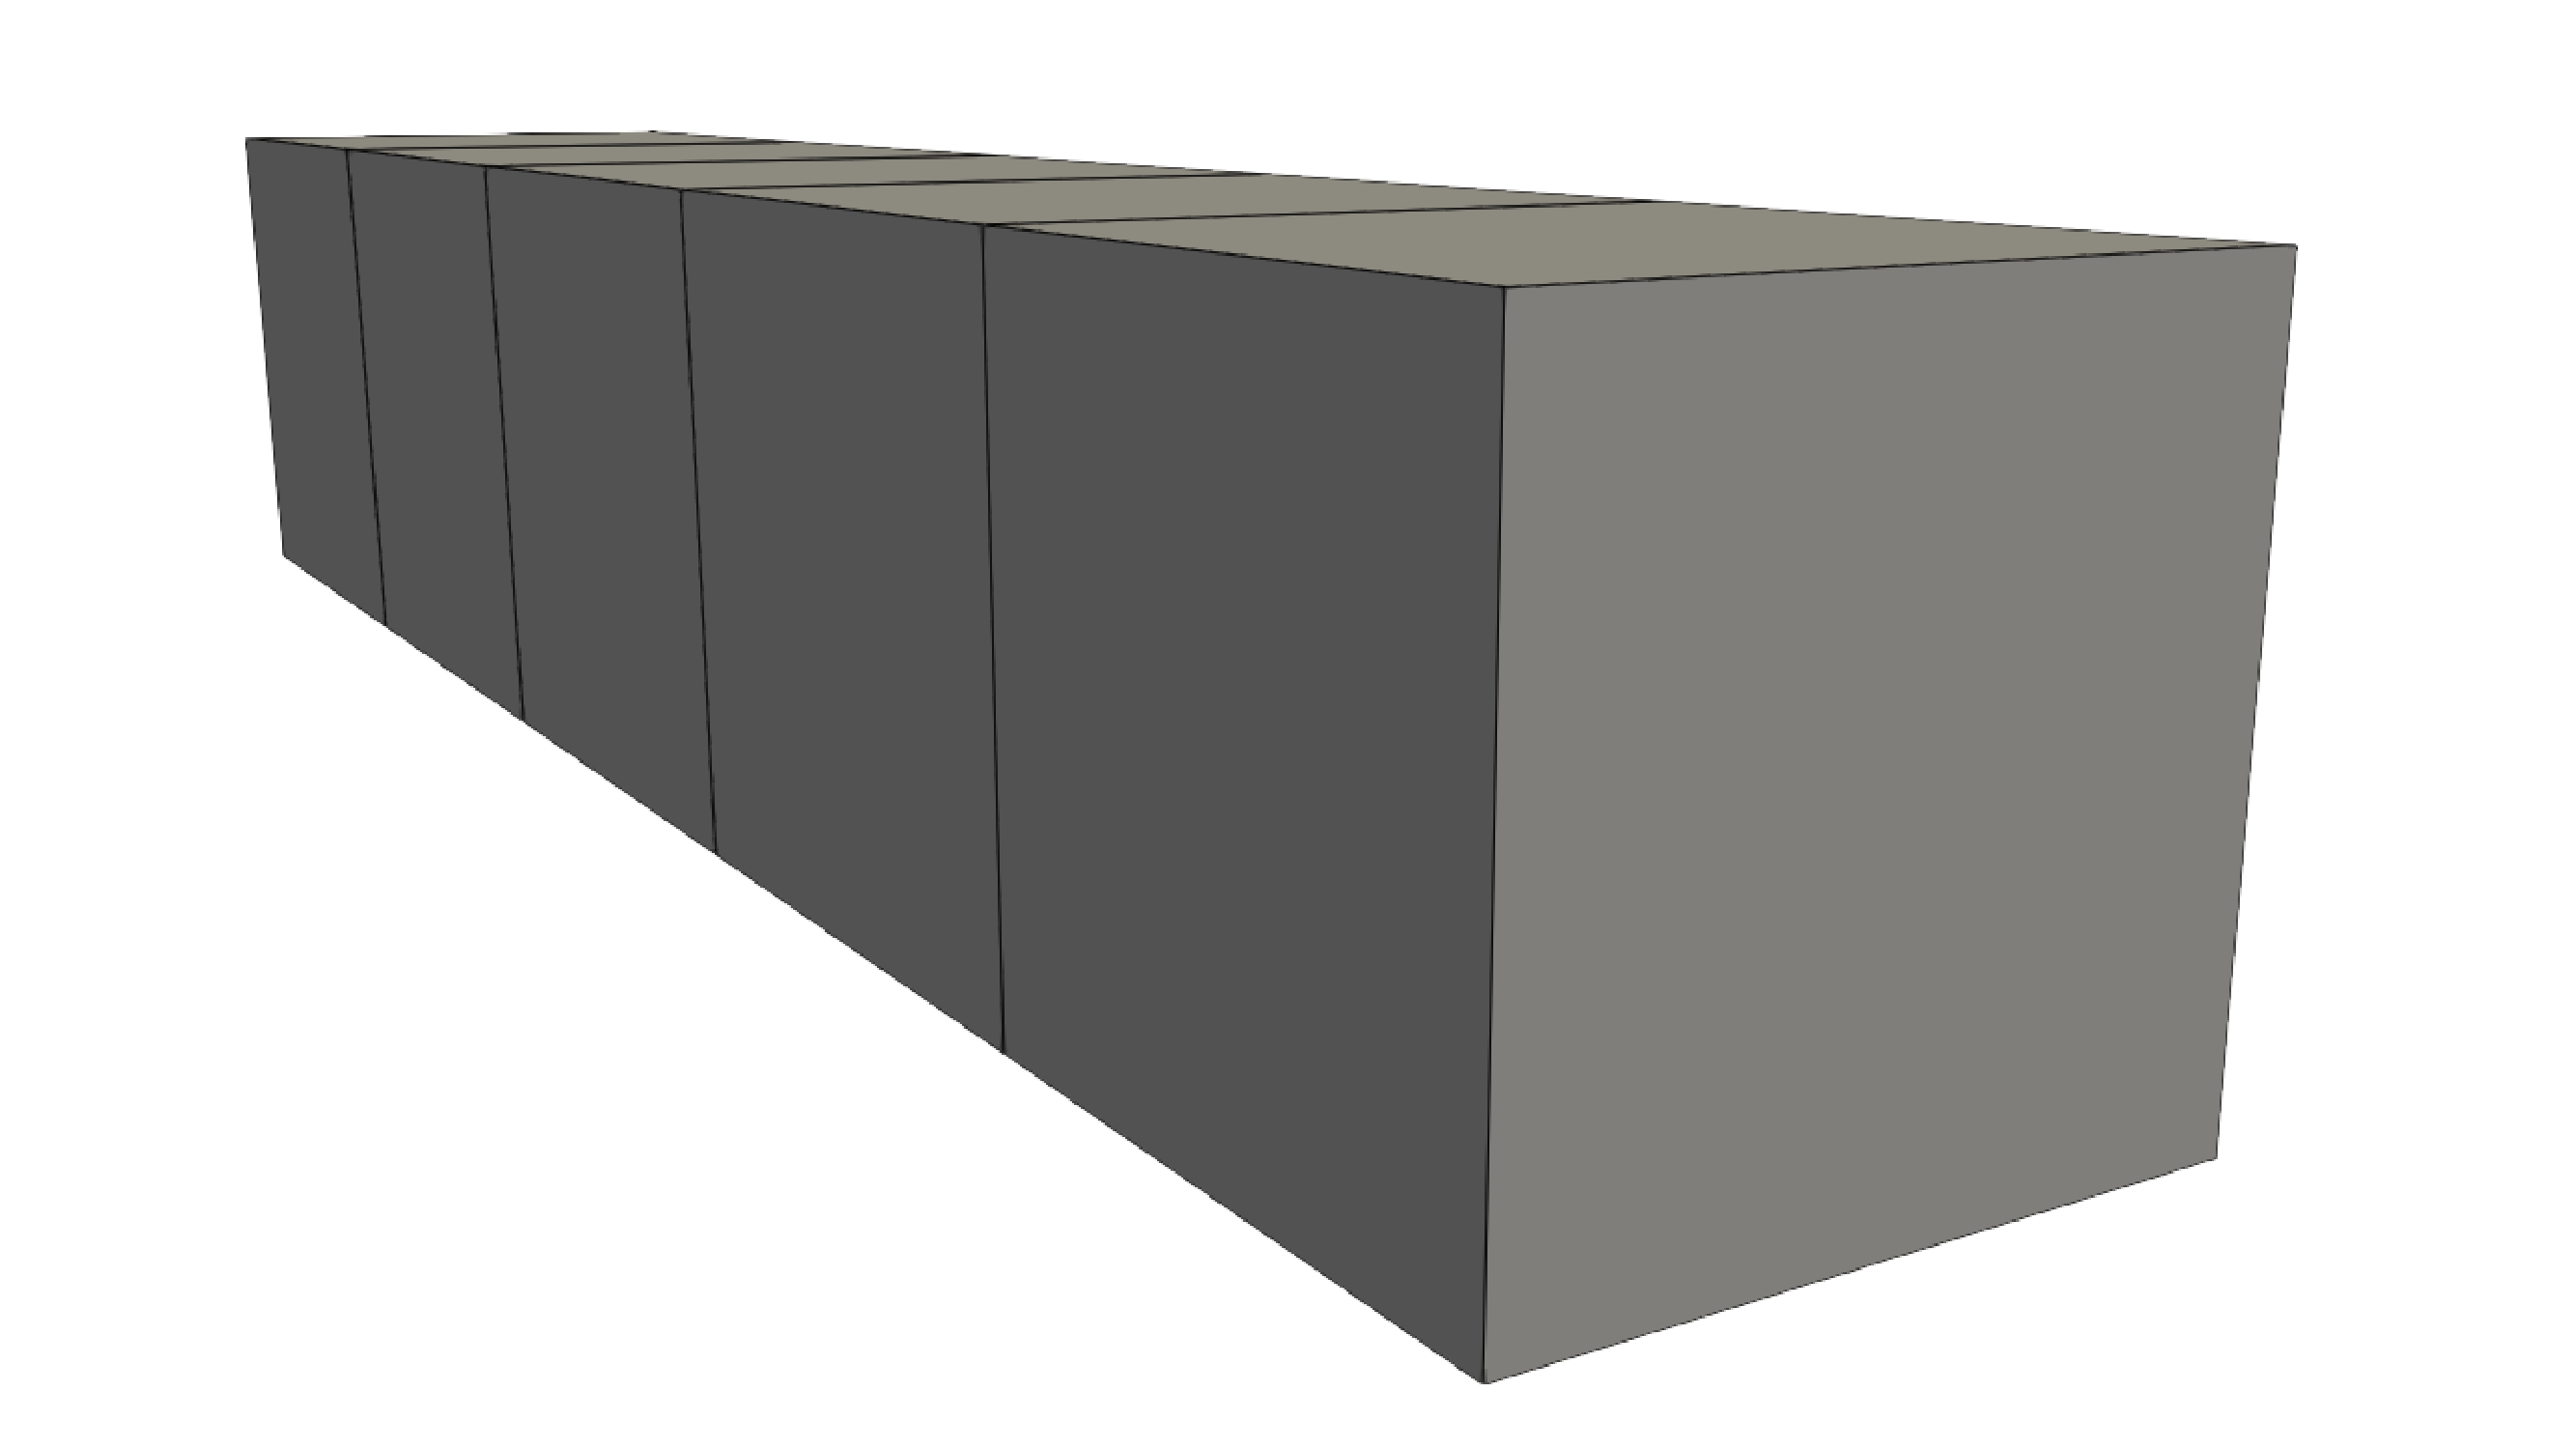
\includegraphics[width=0.35\textwidth]{figs/bishop-mesh1.pdf}} \hfill
	\subfloat[\label{fig:bishop-meshes-b}]{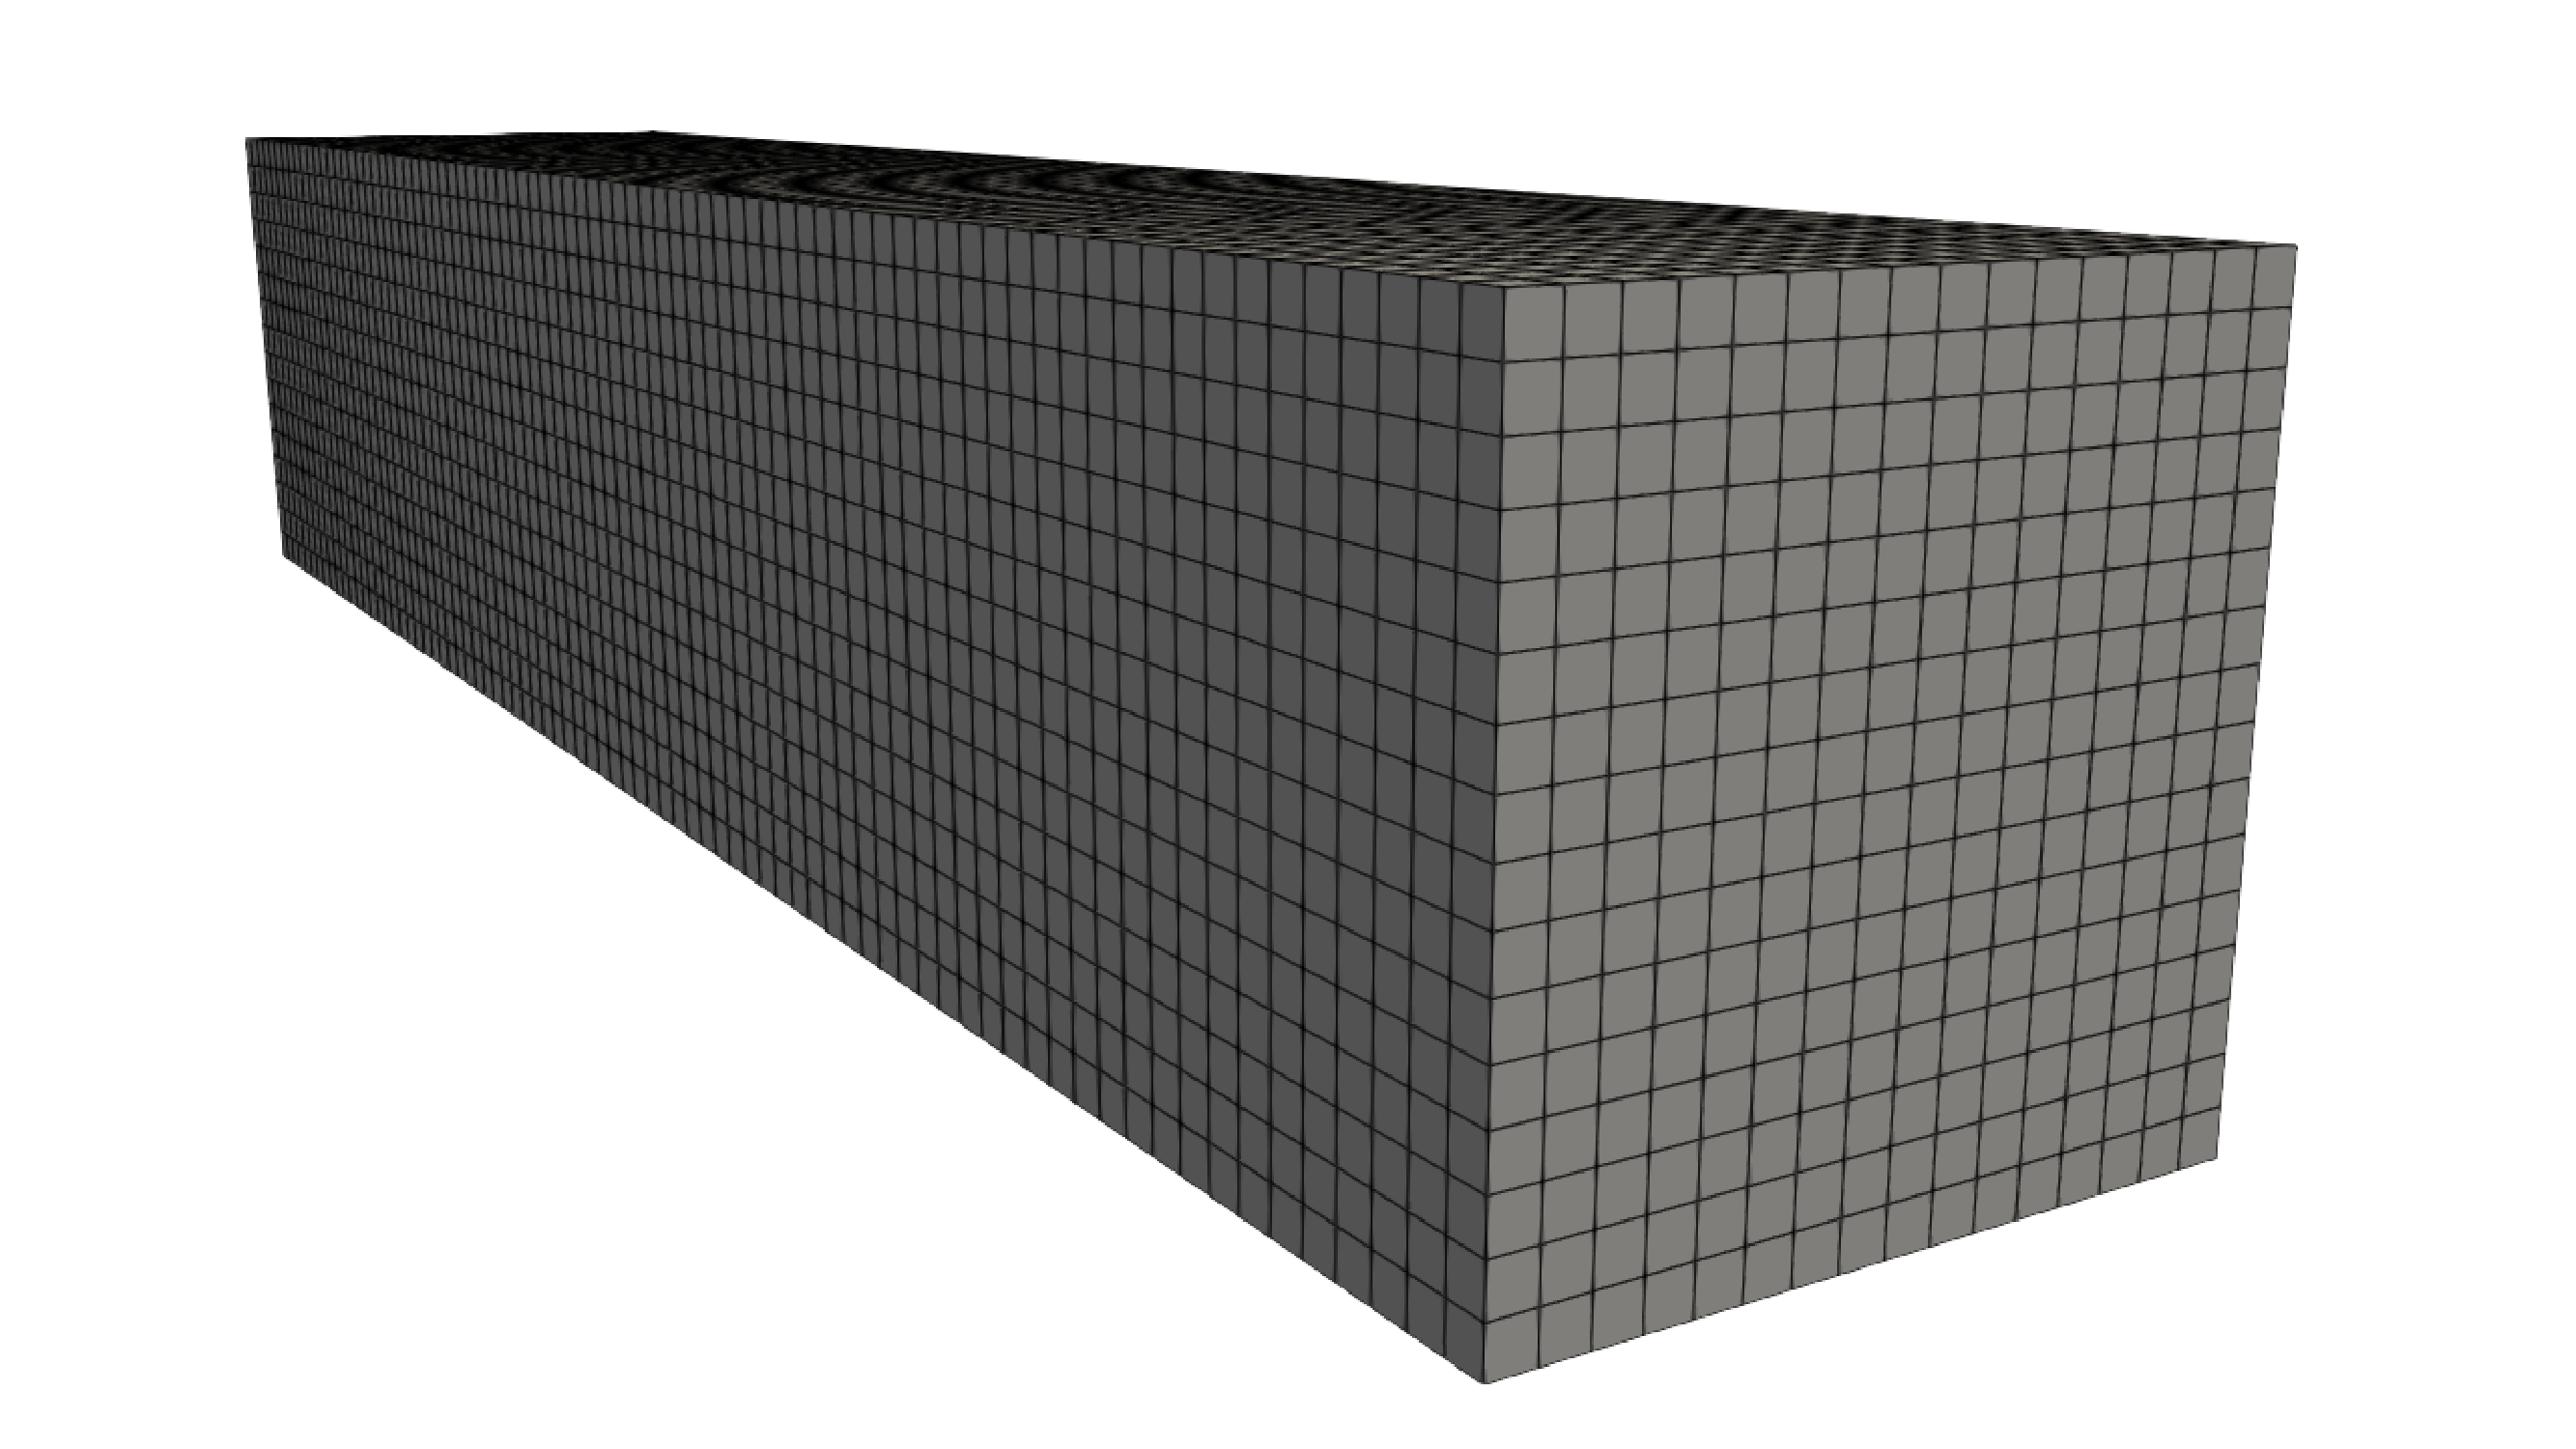
\includegraphics[width=0.35\textwidth]{figs/bishop-mesh2.pdf}}
	\caption{Cantilever beam subjected to an end shear load - geometry (at left), coarsest mesh (at center) and finest mesh (at right)}
	\label{fig:bishop-beam-problem}
\end{figure}

The analytical solutions for the stresses and displacements are available in \cite{bishop2014displacement} and written below:
\vskip-.6cm
\begin{equation} \label{eq:bishop-stress}
	\begin{aligned}
		\sigma_{xx} &= \sigma_{xy} = \sigma_{yy} = 0 \text{,}\\
		\sigma_{zz} &= \frac{F}{I} yz \text{,}\\
		\sigma_{xz} &= \frac{F}{I} \frac{2a^2}{\pi^2}\frac{\nu}{1+\nu} \sum_{n=1}^{\infty} \frac{(-1)^n}{n^2} \text{sin}\left(n\pi x/a\right) \frac{\text{sinh}\left( n\pi y/a \right)}{\text{cosh}\left( n\pi b/a \right)} \text{,}\\
		\sigma_{yz} &= \frac{F}{I} \frac{b^2-y^2}{2} + \frac{F}{I}\frac{\nu}{1+\nu} \left[ \frac{3x^2-a^2}{6} - \frac{2a^2}{\pi^2} \sum_{n=1}^{\infty} \frac{(-1)^n}{n^2} \text{cos}\left(n\pi x/a\right) \frac{\text{cosh}\left( n\pi y/a \right)}{\text{cosh}\left( n\pi b/a \right)}  \right]\text{,}\\
	\end{aligned}
\end{equation}
and
\vskip-.6cm
\begin{equation} \label{eq:bishop-displacement}
	\begin{split}
		u_x & = -\frac{F\nu}{EI} xyz \text{,}\\
		u_y & = \frac{F}{EI} \left[ \frac{\nu}{2}\left(x^2-y^2\right)z - \frac{1}{6}z^3 \right] \text{,}\\
		u_z & = \frac{F}{EI} \left[ \frac{1}{2y}\left(\nu x^2+z^2\right)z + \frac{1}{6}\nu y^3 +(1+\nu) \left(b^2 y -\frac{1}{3}y^3\right) -\frac{1}{3}a^2 \nu y \right. \\
		&\qquad\quad \left.-\frac{4a^3\nu}{\pi^3} \sum_{n=1}^{\infty} \frac{(-1)^n}{n^3} \text{cos}\left(n\pi x/a\right) \frac{\text{sinh}\left( n\pi y/a \right)}{\text{cosh}\left( n\pi b/a \right)} \right] \text{.}
	\end{split}
\end{equation}
\noindent where $I=4ab^3/3$ is the second moment of area about the $x$-axis, and the series above are evaluated with a finite number of terms $n=5$.

The beam is discretized using hexahedral elements, where the element size is computed as $h_e=1/2^{N}$, with $N=\{0,1,2,3,4\}$. The coarsest ($h_e=1$) and finest ($h_e=0.0625$) meshes are shown in Figures \ref{fig:bishop-meshes-a}-\ref{fig:bishop-meshes-b}. A convergence test is performed for displacement, pressure, stress and mass conservation, where the error is computed according to the $L^2$ norm defined as:
\vskip-.3cm
\begin{equation} \label{eq:bishop-errors}
	\left\| \mathbf{u}^h-\mathbf{u}_{exact}  \right\|_{L^2} \doteq \left[ \sum_{e=1}^{n} \int_{\Omega_e} \left(\mathbf{u} - \mathbf{u}^h\right)^2 d\Omega_e\right]^{1/2} \text{.}
\end{equation}

The results are depicted in Figures \ref{fig:bishop-convergence-nu-03}-\ref{fig:bishop-convergence-nu-05} and present optimal convergence rates of $k+1$ for the displacement and $k$ for the remaining variables independently of the poisson coefficient. This is a nice feature as many formulations present a locking phenomena under quasi and full incompressibility. For the incompressible case ($\nu=0.5$), a divergence free displacement field is obtained even for the coarsest mesh thanks to the stable pair $H(\text{div},\Omega)$-$L^2(\Omega)$, with the error bounded to the machine precision.

\begin{figure} [!htb]
    \centering
    % \subfloat[]{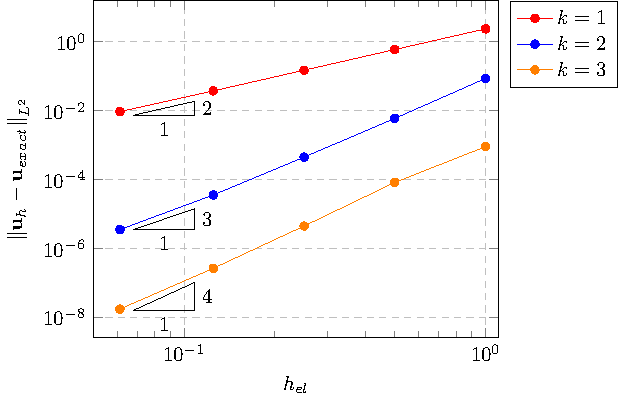
\includegraphics[trim={0cm 0cm 2.0cm 0cm},clip,width=0.27\textwidth]{figs/bishop-disp-03.pdf}} \hfill
    % \subfloat[]{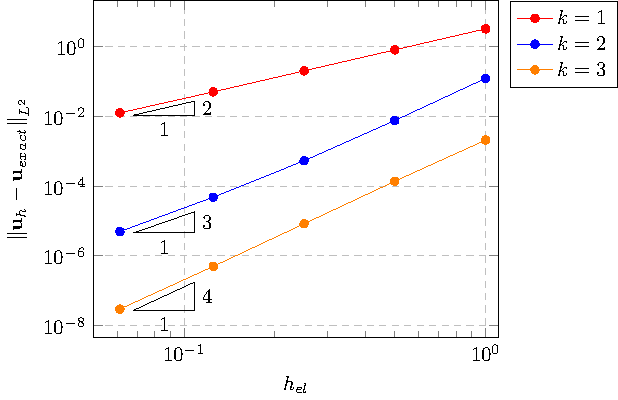
\includegraphics[trim={0cm 0cm 2.0cm 0cm},clip,width=0.27\textwidth]{figs/bishop-disp-04999.pdf}} \hfill
    % \subfloat[]{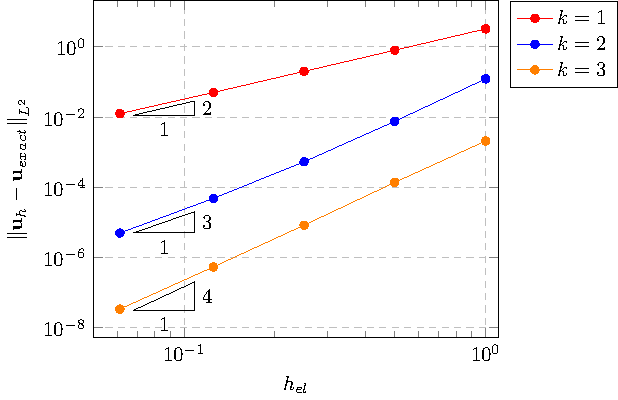
\includegraphics[trim={0cm 0cm 2.0cm 0cm},clip,width=0.27\textwidth]{figs/bishop-disp-05.pdf}}
    % 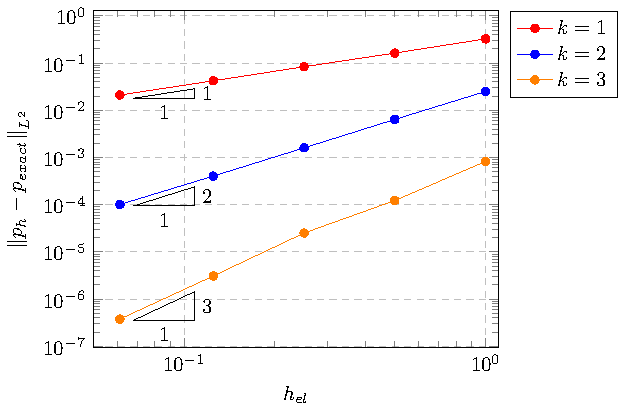
\includegraphics[trim={8.5cm 0cm 0cm 0cm},clip,scale=0.7]{figs/bishop-pres-03.pdf}
    \subfloat[]{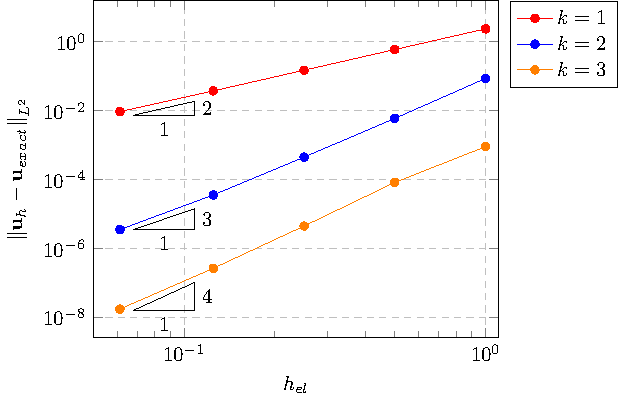
\includegraphics[trim={0cm 0cm 2.0cm 0cm},clip,scale=0.75]{figs/bishop-disp-03.pdf}} \hfill
    \subfloat[]{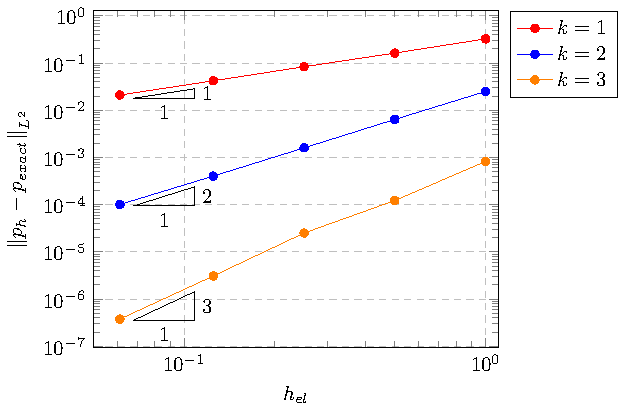
\includegraphics[trim={0cm 0cm 2.0cm 0cm},clip,scale=0.75]{figs/bishop-pres-03.pdf}}
    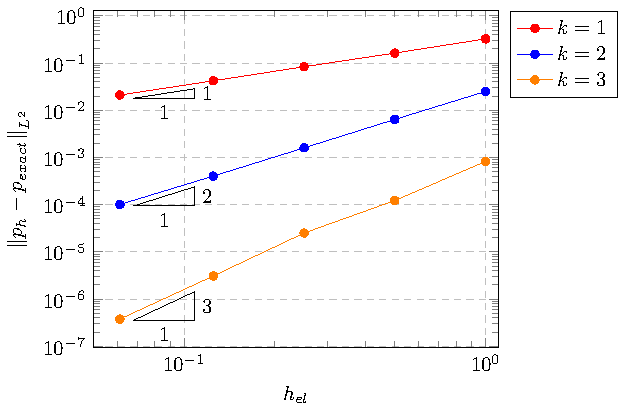
\includegraphics[trim={8.5cm 0cm 0cm 0cm},clip,scale=0.75]{figs/bishop-pres-03.pdf}
    \subfloat[]{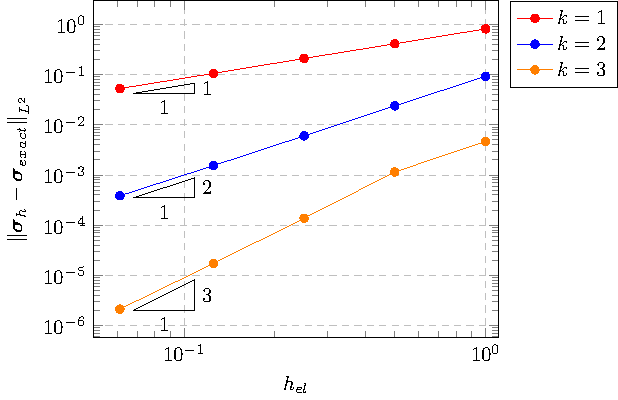
\includegraphics[trim={0cm 0cm 2.0cm 0cm},clip,scale=0.75]{figs/bishop-stress-03.pdf}} \hfill
    \subfloat[]{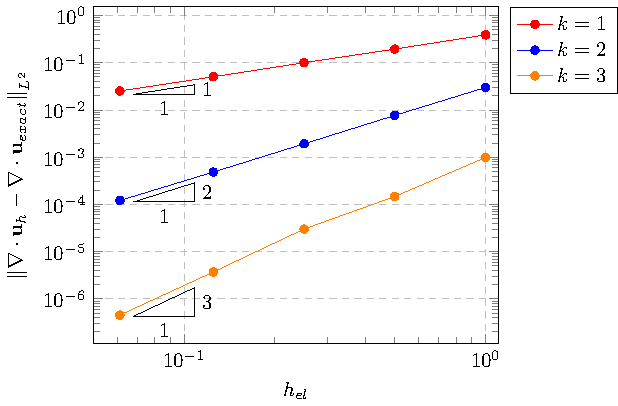
\includegraphics[trim={0cm 0cm 2.0cm 0cm},clip,scale=0.75]{figs/bishop-div-03.pdf}}
    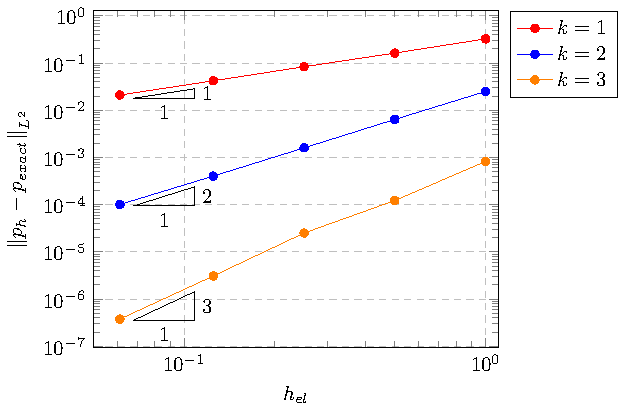
\includegraphics[trim={8.5cm 0cm 0cm 0cm},clip,scale=0.75]{figs/bishop-pres-03.pdf}
    \caption{Cantilever beam subjected to an end shear load - convergence analysis for the compressible case ($\nu=0.30$)}
    \label{fig:bishop-convergence-nu-03}
\end{figure}

\begin{figure} [!htb]
    \centering
    \subfloat[\label{fig:bishop-convergence-nu-04999-a}Displacement]{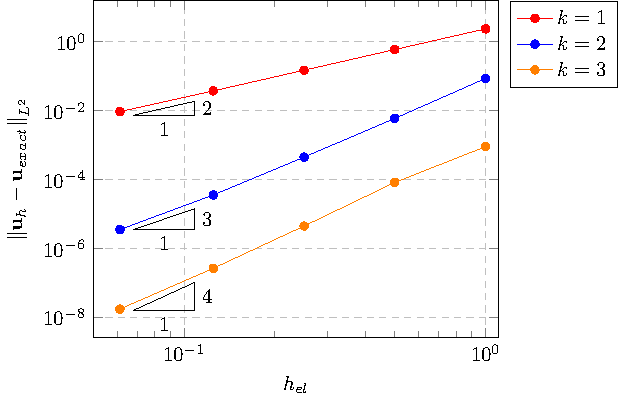
\includegraphics[trim={0cm 0cm 2.0cm 0cm},clip,scale=0.75]{figs/bishop-disp-03.pdf}} \hfill
    \subfloat[\label{fig:bishop-convergence-nu-04999-b}Pressure]{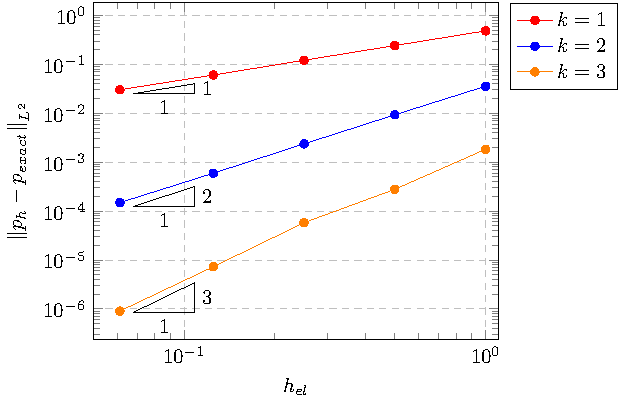
\includegraphics[trim={0cm 0cm 2.0cm 0cm},clip,scale=0.75]{figs/bishop-pres-04999.pdf}}
    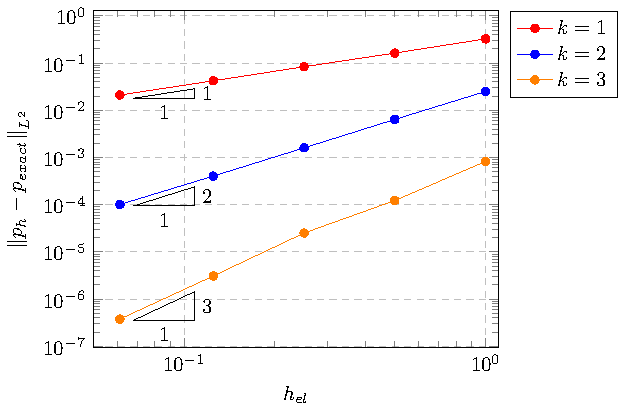
\includegraphics[trim={8.5cm 0cm 0cm 0cm},clip,scale=0.75]{figs/bishop-pres-03.pdf}
    \subfloat[\label{fig:bishop-convergence-nu-04999-c}Stress]{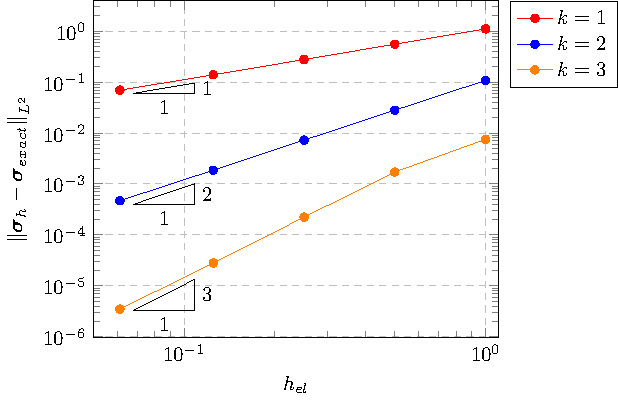
\includegraphics[trim={0cm 0cm 2.0cm 0cm},clip,scale=0.75]{figs/bishop-stress-04999.pdf}} \hfill
    \subfloat[\label{fig:bishop-convergence-nu-04999-d}Divergence]{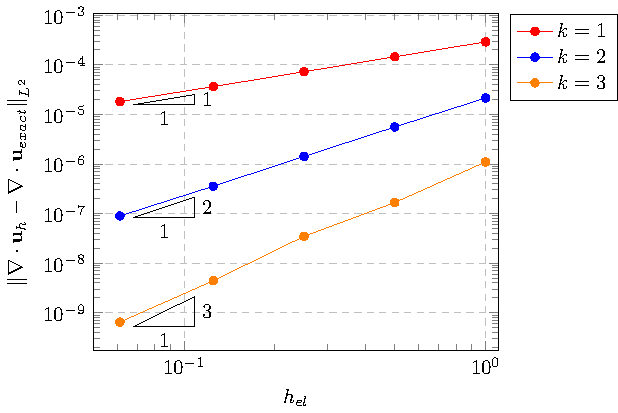
\includegraphics[trim={0cm 0cm 2.0cm 0cm},clip,scale=0.75]{figs/bishop-div-04999.pdf}}
    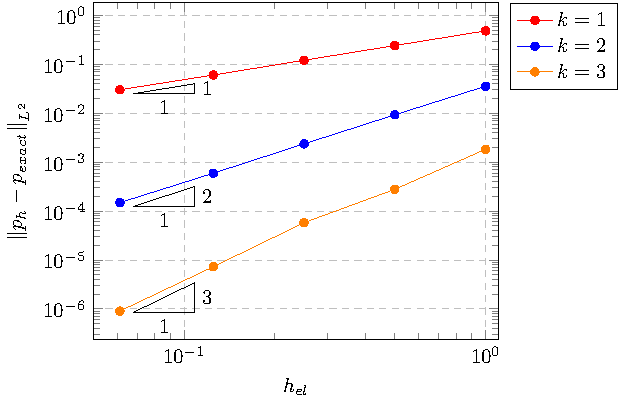
\includegraphics[trim={8.5cm 0cm 0cm 0cm},clip,scale=0.75]{figs/bishop-pres-04999.pdf}
    \caption{Cantilever beam subjected to an end shear load - convergence analysis for the quasi-incompressible case ($\nu=0.4999$)}
    \label{fig:bishop-convergence-nu-04999}
\end{figure}

\begin{figure} [!htb]
    \centering
    \subfloat[\label{fig:bishop-convergence-nu-05-a}Displacement]{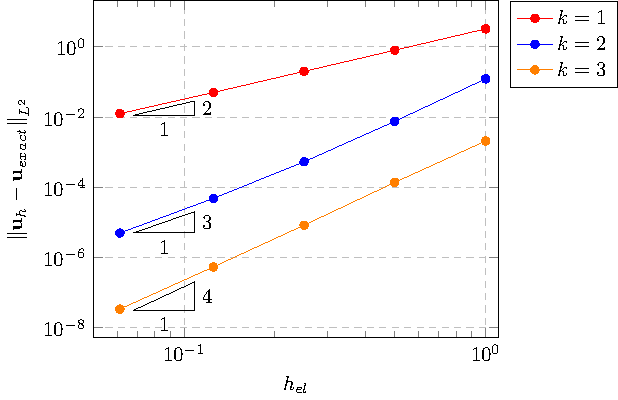
\includegraphics[trim={0cm 0cm 2.0cm 0cm},clip,scale=0.75]{figs/bishop-disp-05.pdf}} \hfill
    \subfloat[\label{fig:bishop-convergence-nu-05-b}Pressure]{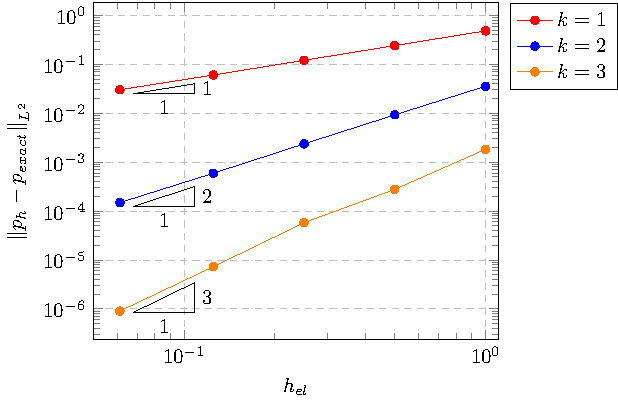
\includegraphics[trim={0cm 0cm 2.0cm 0cm},clip,scale=0.75]{figs/bishop-pres-05.pdf}}
    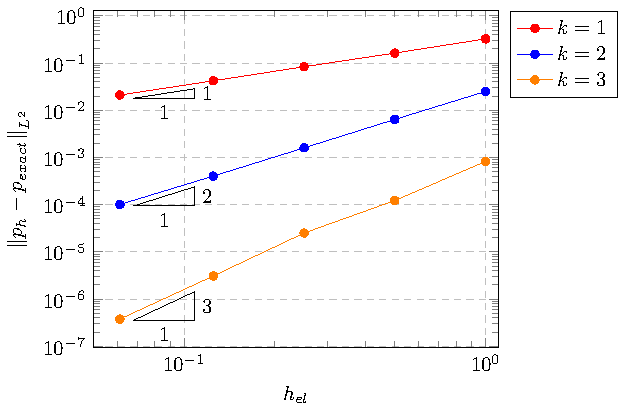
\includegraphics[trim={8.5cm 0cm 0cm 0cm},clip,scale=0.75]{figs/bishop-pres-03.pdf}
    \subfloat[\label{fig:bishop-convergence-nu-05-c}Stress]{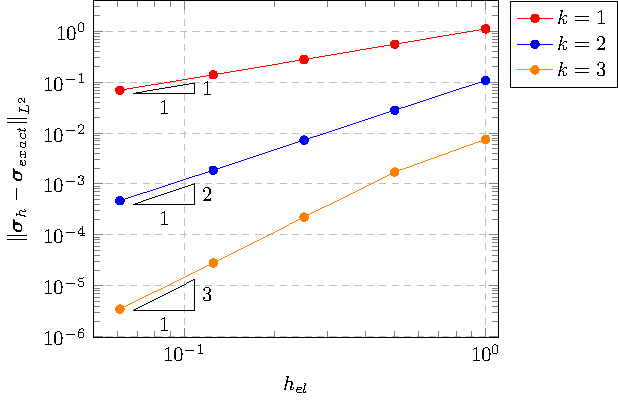
\includegraphics[trim={0cm 0cm 2.0cm 0cm},clip,scale=0.75]{figs/bishop-stress-05.pdf}} \hfill
    \subfloat[\label{fig:bishop-convergence-nu-05-d}Divergence]{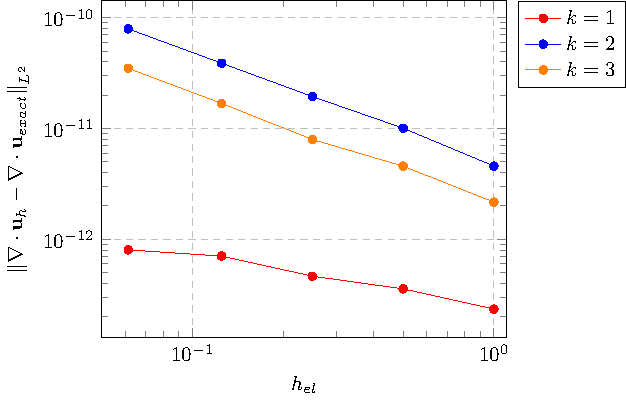
\includegraphics[trim={0cm 0cm 2.0cm 0cm},clip,scale=0.75]{figs/bishop-div-05.pdf}}
    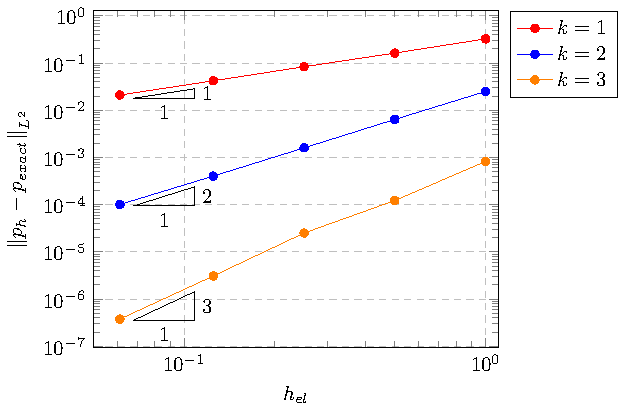
\includegraphics[trim={8.5cm 0cm 0cm 0cm},clip,scale=0.75]{figs/bishop-pres-03.pdf}
    \caption{Cantilever beam subjected to an end shear load - convergence analysis for the incompressible case ($\nu=0.5$)}
    \label{fig:bishop-convergence-nu-05}
\end{figure}

Figure \ref{fig:bishop-snapshot} plots the displacement, pressure, normal and shear stresses distributions obtained with the finest mesh using $k=2$ over the deformed configuration of the beam for the compressible case. The results qualitatively agrees with the reference solution of \cite{bishop2014displacement}.

\begin{figure} [!htb]
    \centering
    \subfloat[\label{fig:bishop-snapshot-a}Displacement]{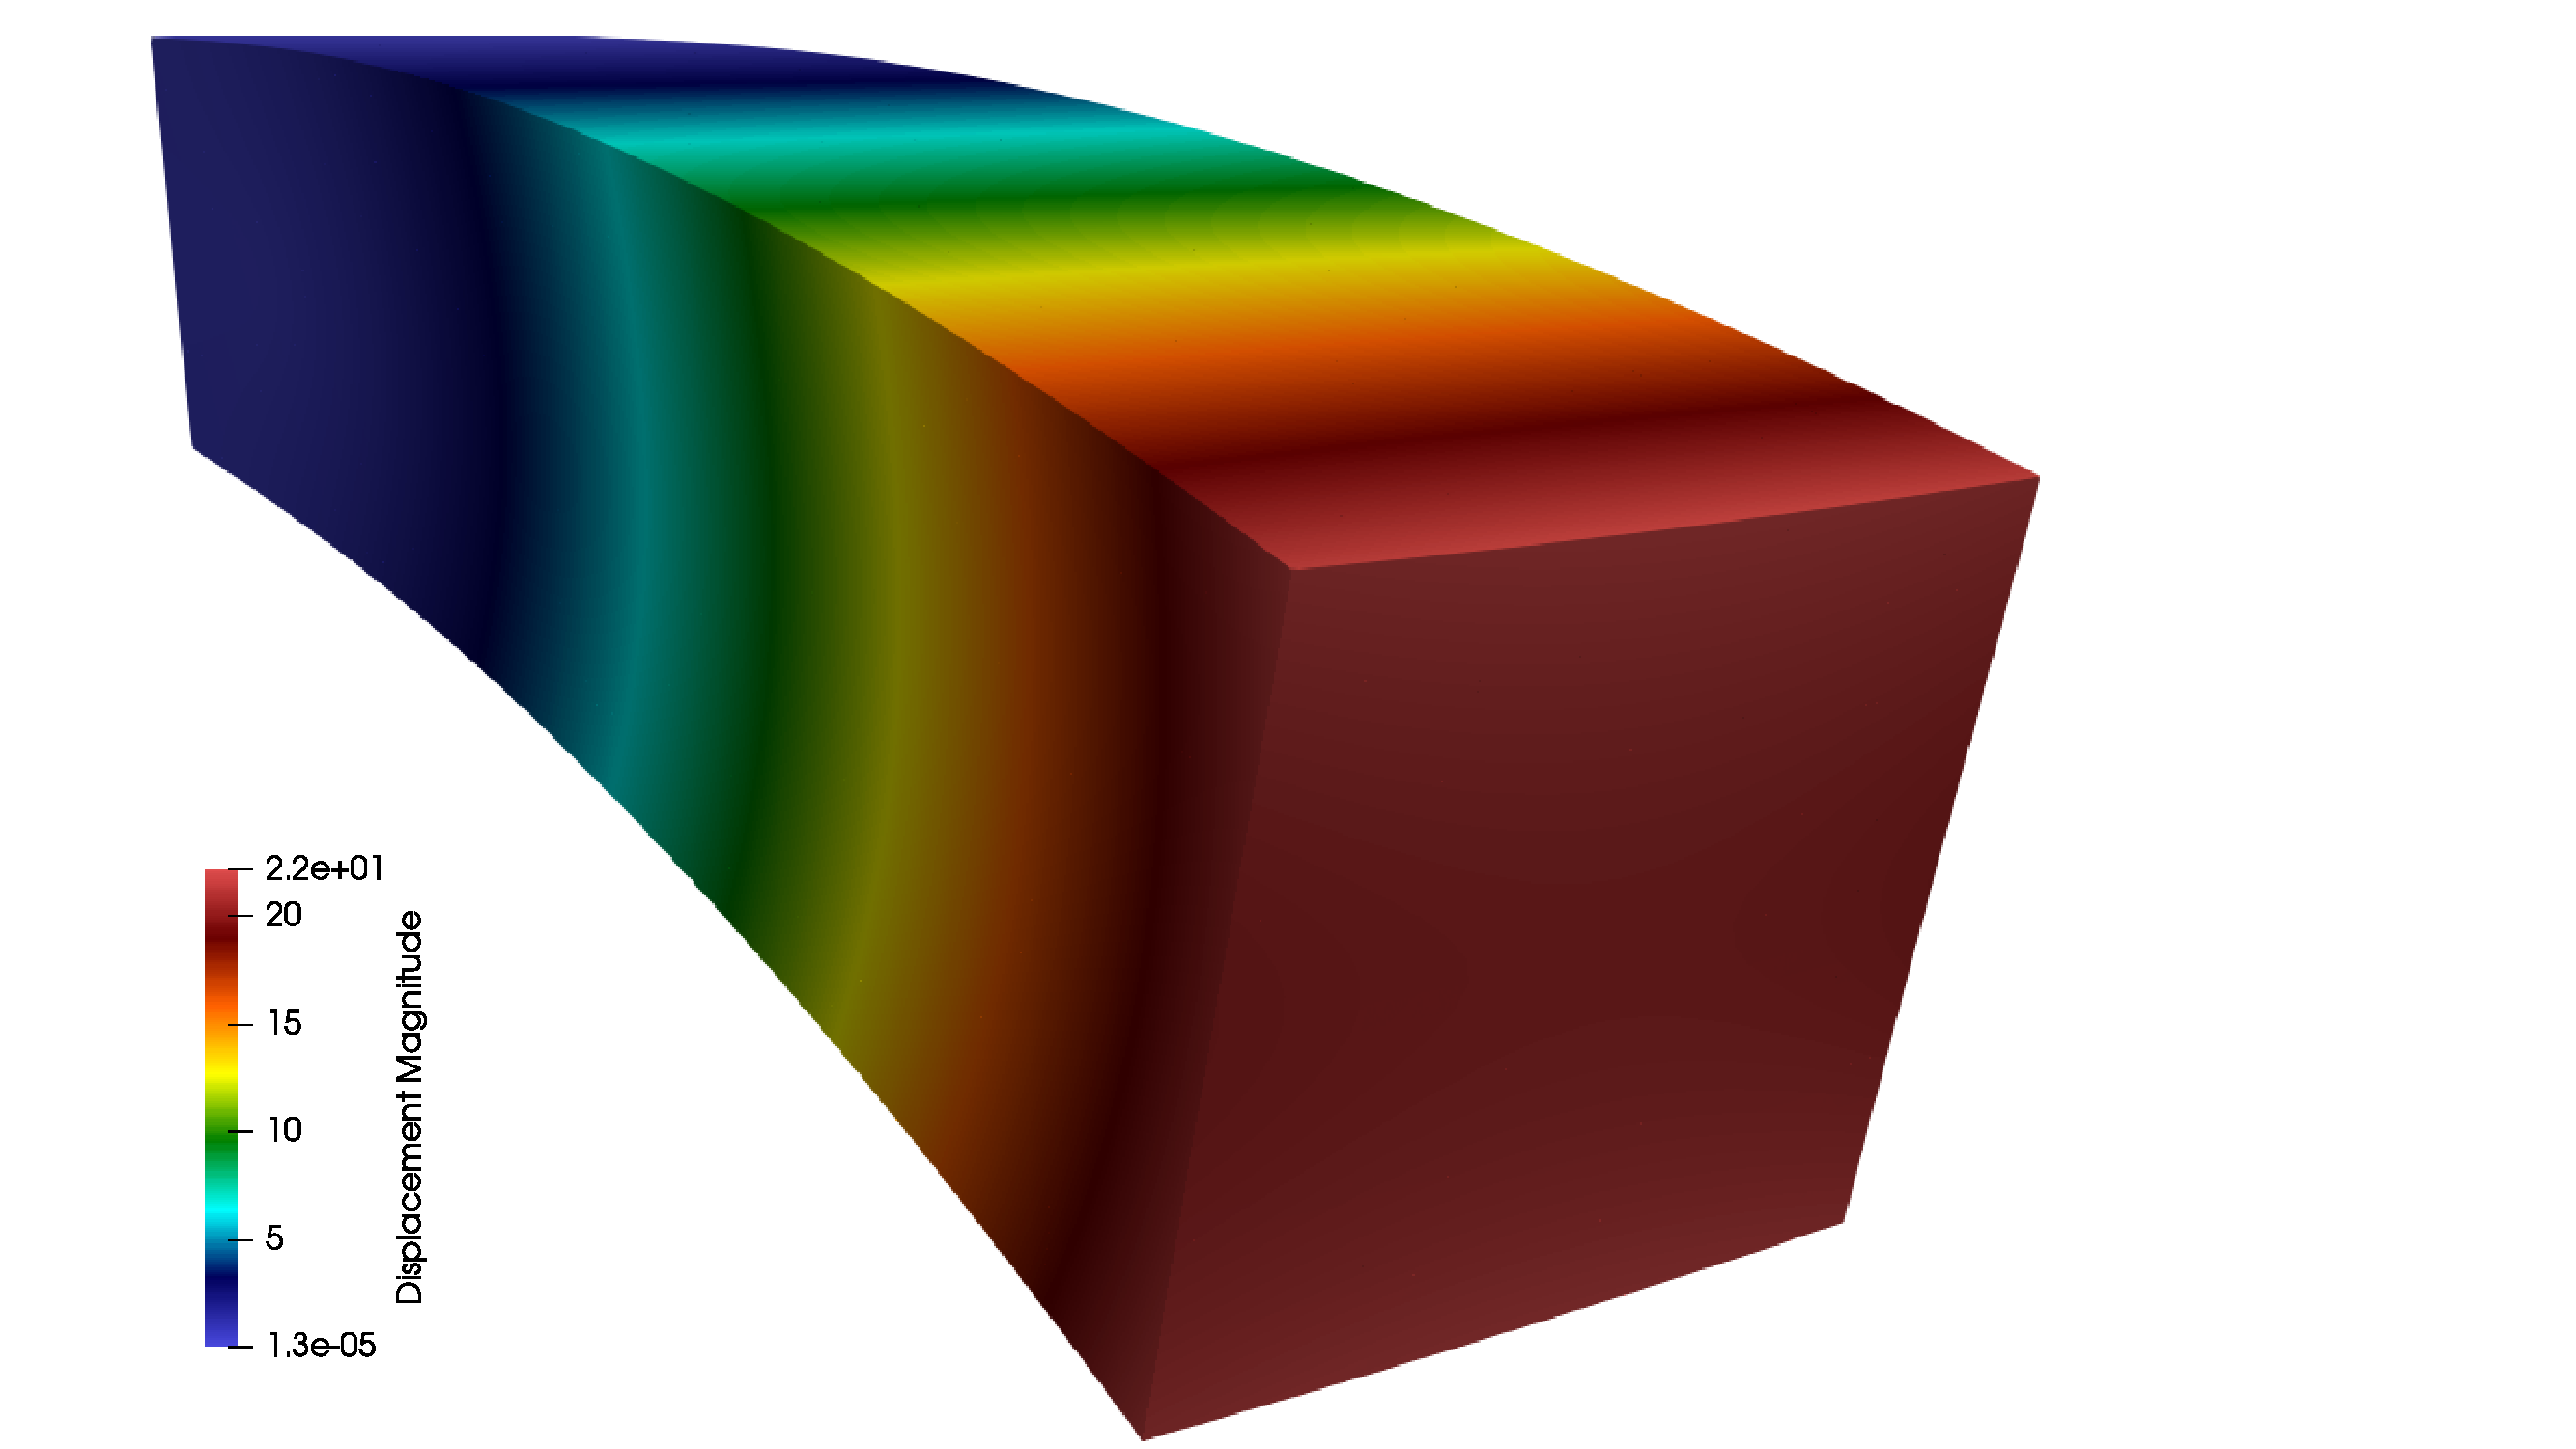
\includegraphics[trim={2.5cm 0cm 9.2cm 0cm},clip,scale=0.2]{figs/bishop-snapshot-a.pdf}} \hfill
    \subfloat[\label{fig:bishop-snapshot-b}Pressure]{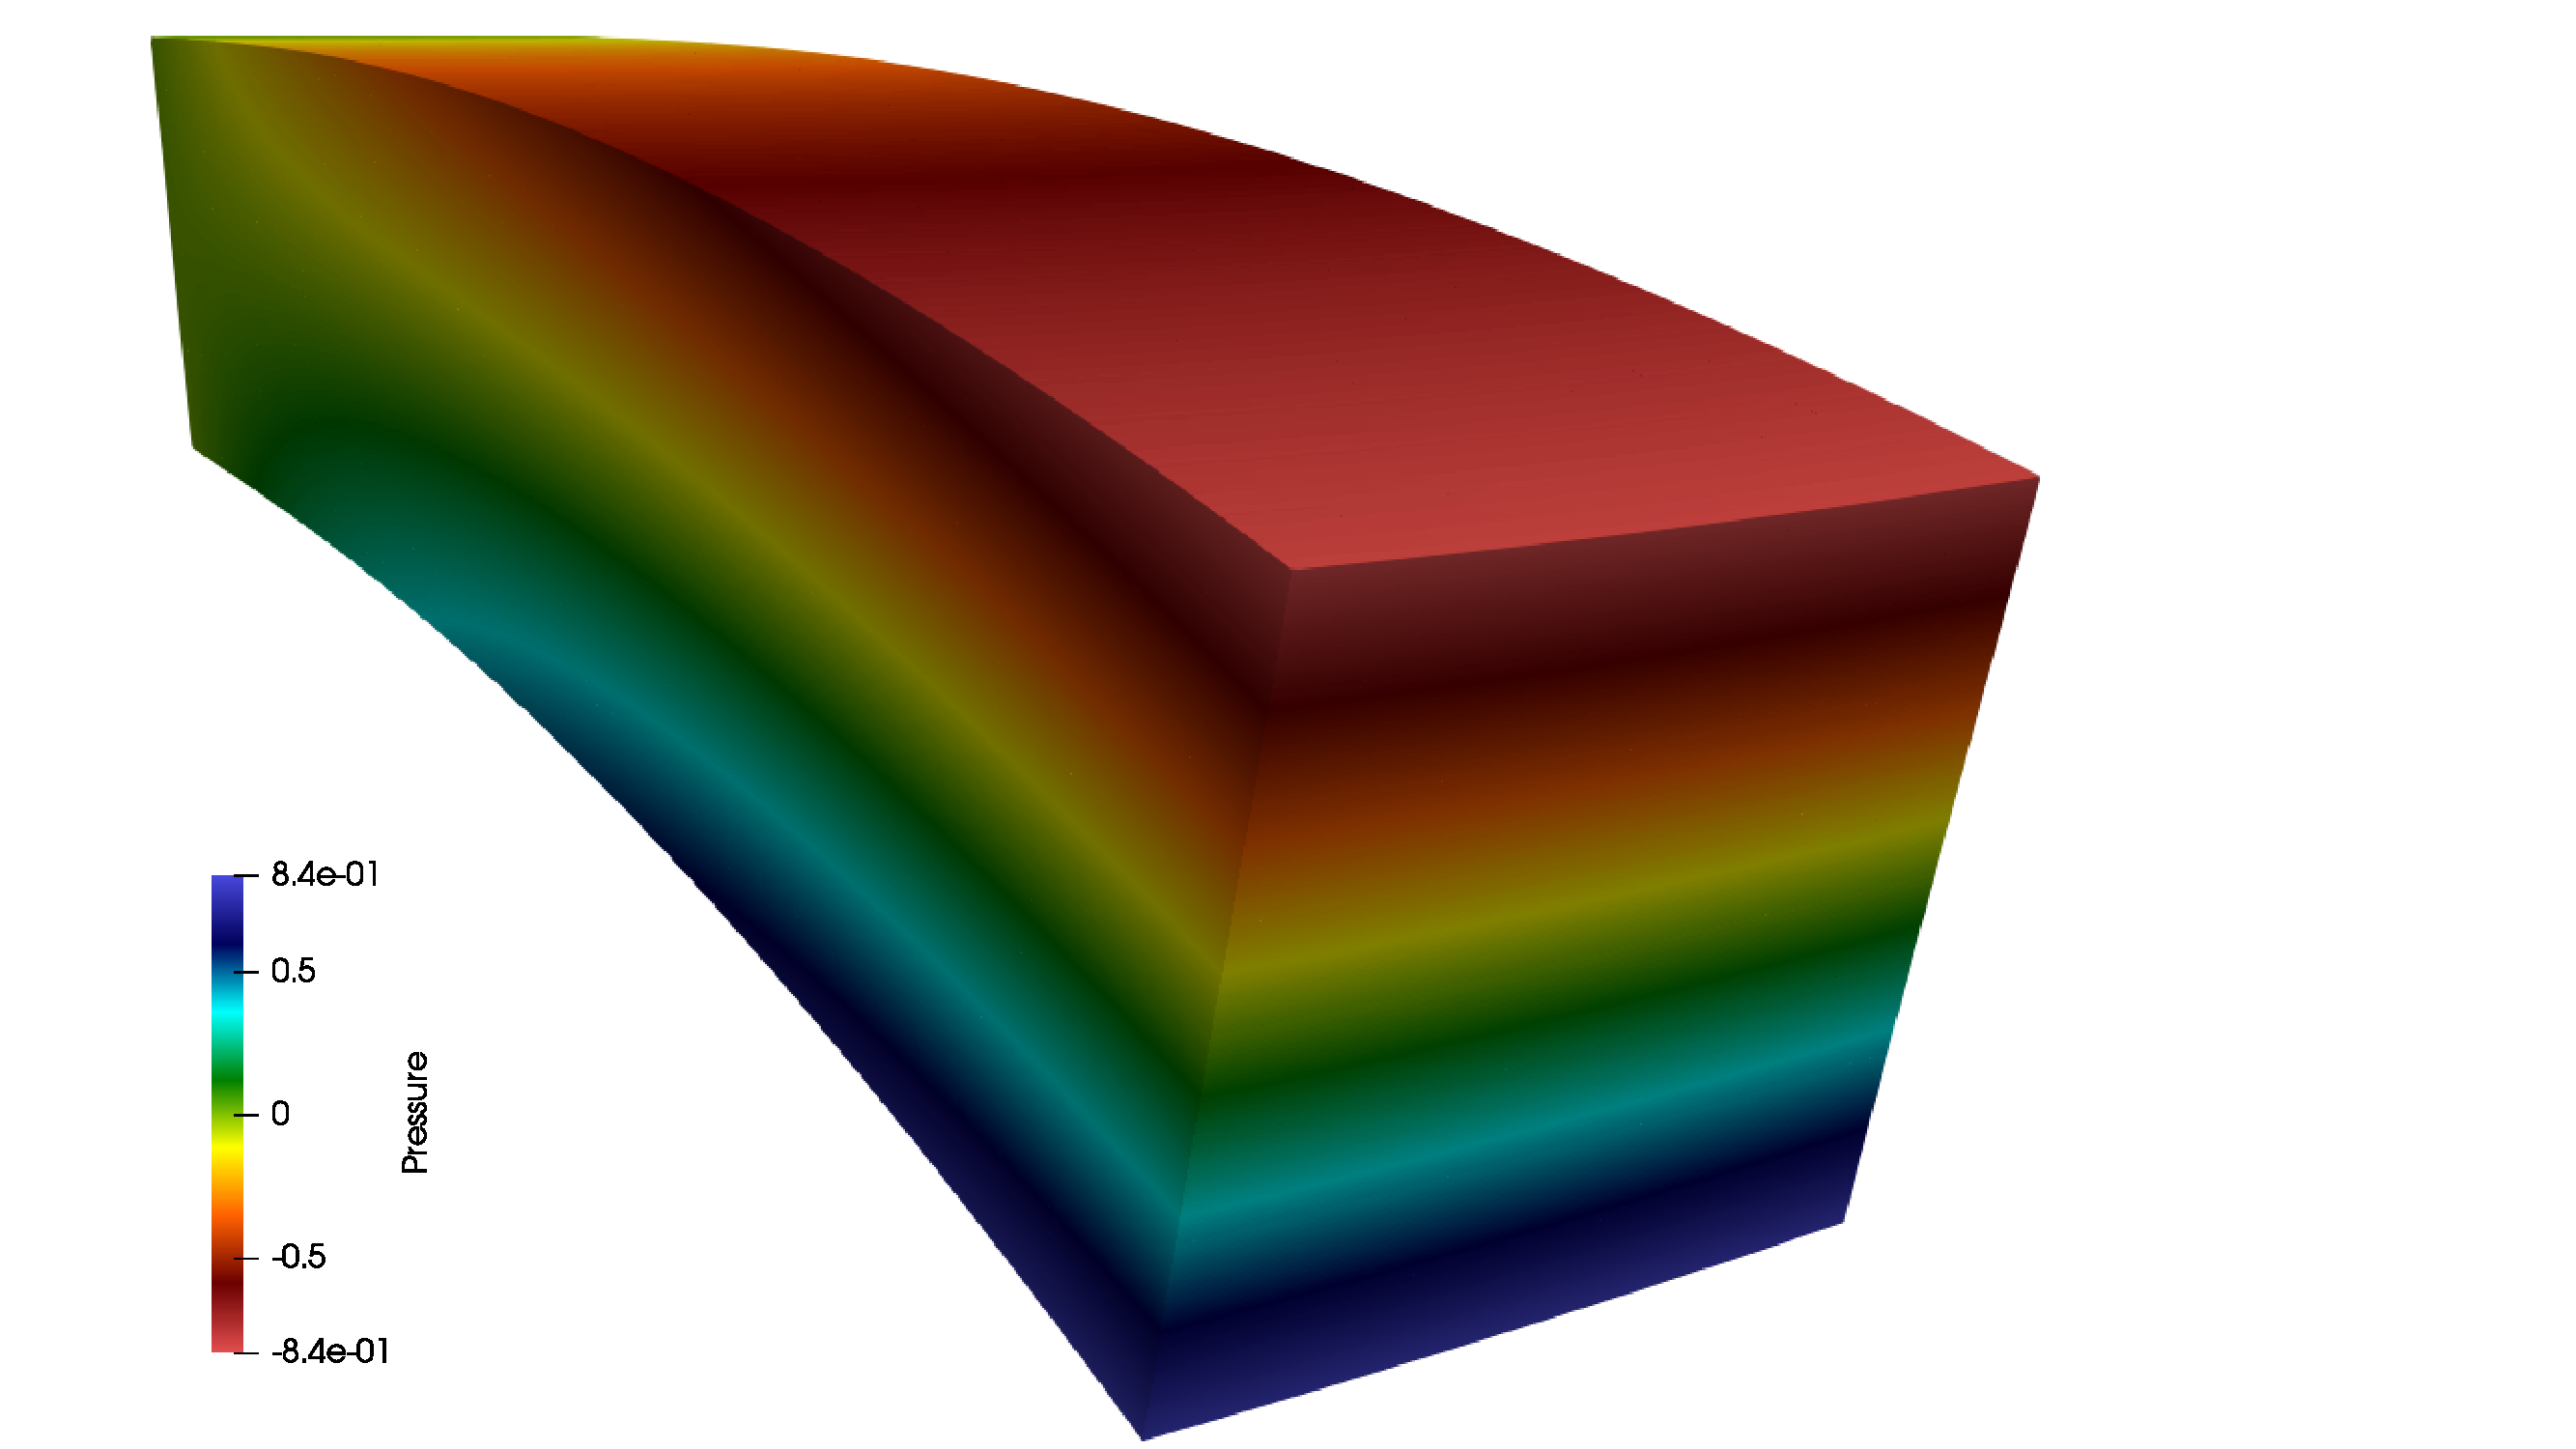
\includegraphics[trim={2.5cm 0cm 9.2cm 0cm},clip,scale=0.2]{figs/bishop-snapshot-b.pdf}} \\
    \subfloat[\label{fig:bishop-snapshot-c}Normal stress $\sigma_{zz}$]{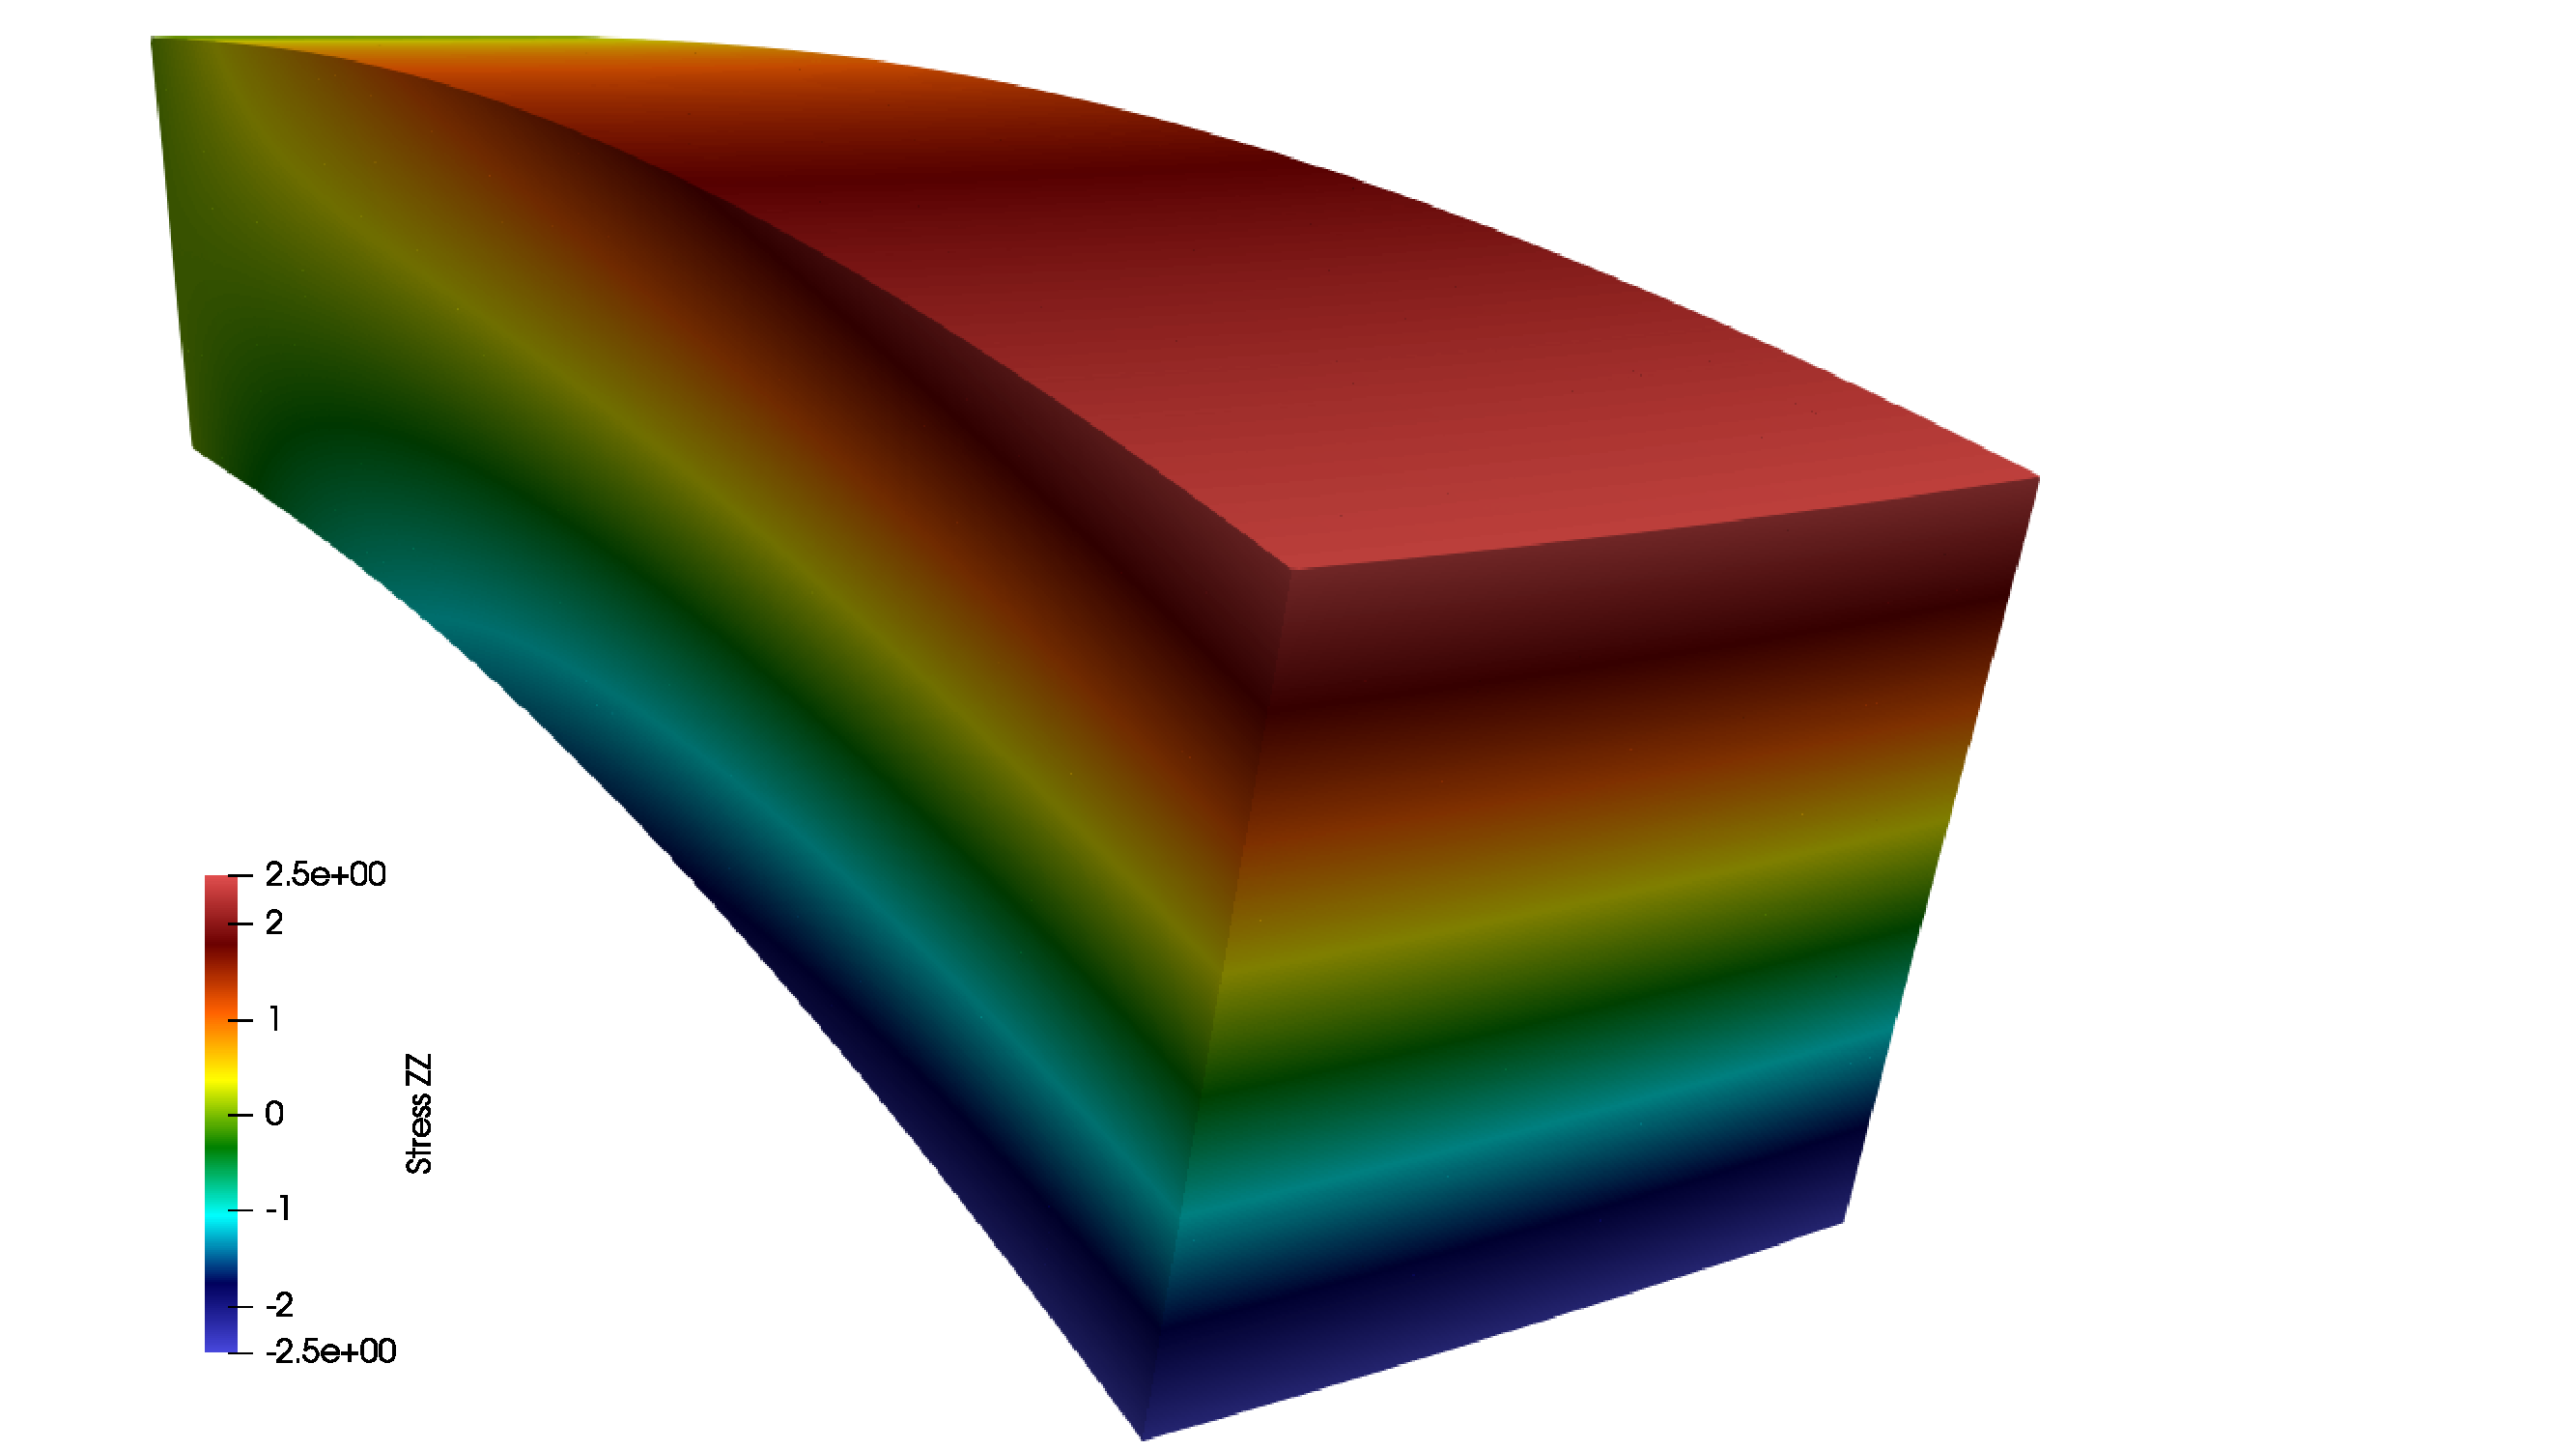
\includegraphics[trim={2.5cm 0cm 9.2cm 0cm},clip,scale=0.2]{figs/bishop-snapshot-c.pdf}} \hfill
    \subfloat[\label{fig:bishop-snapshot-d}Shear stress $\sigma_{yz}$]{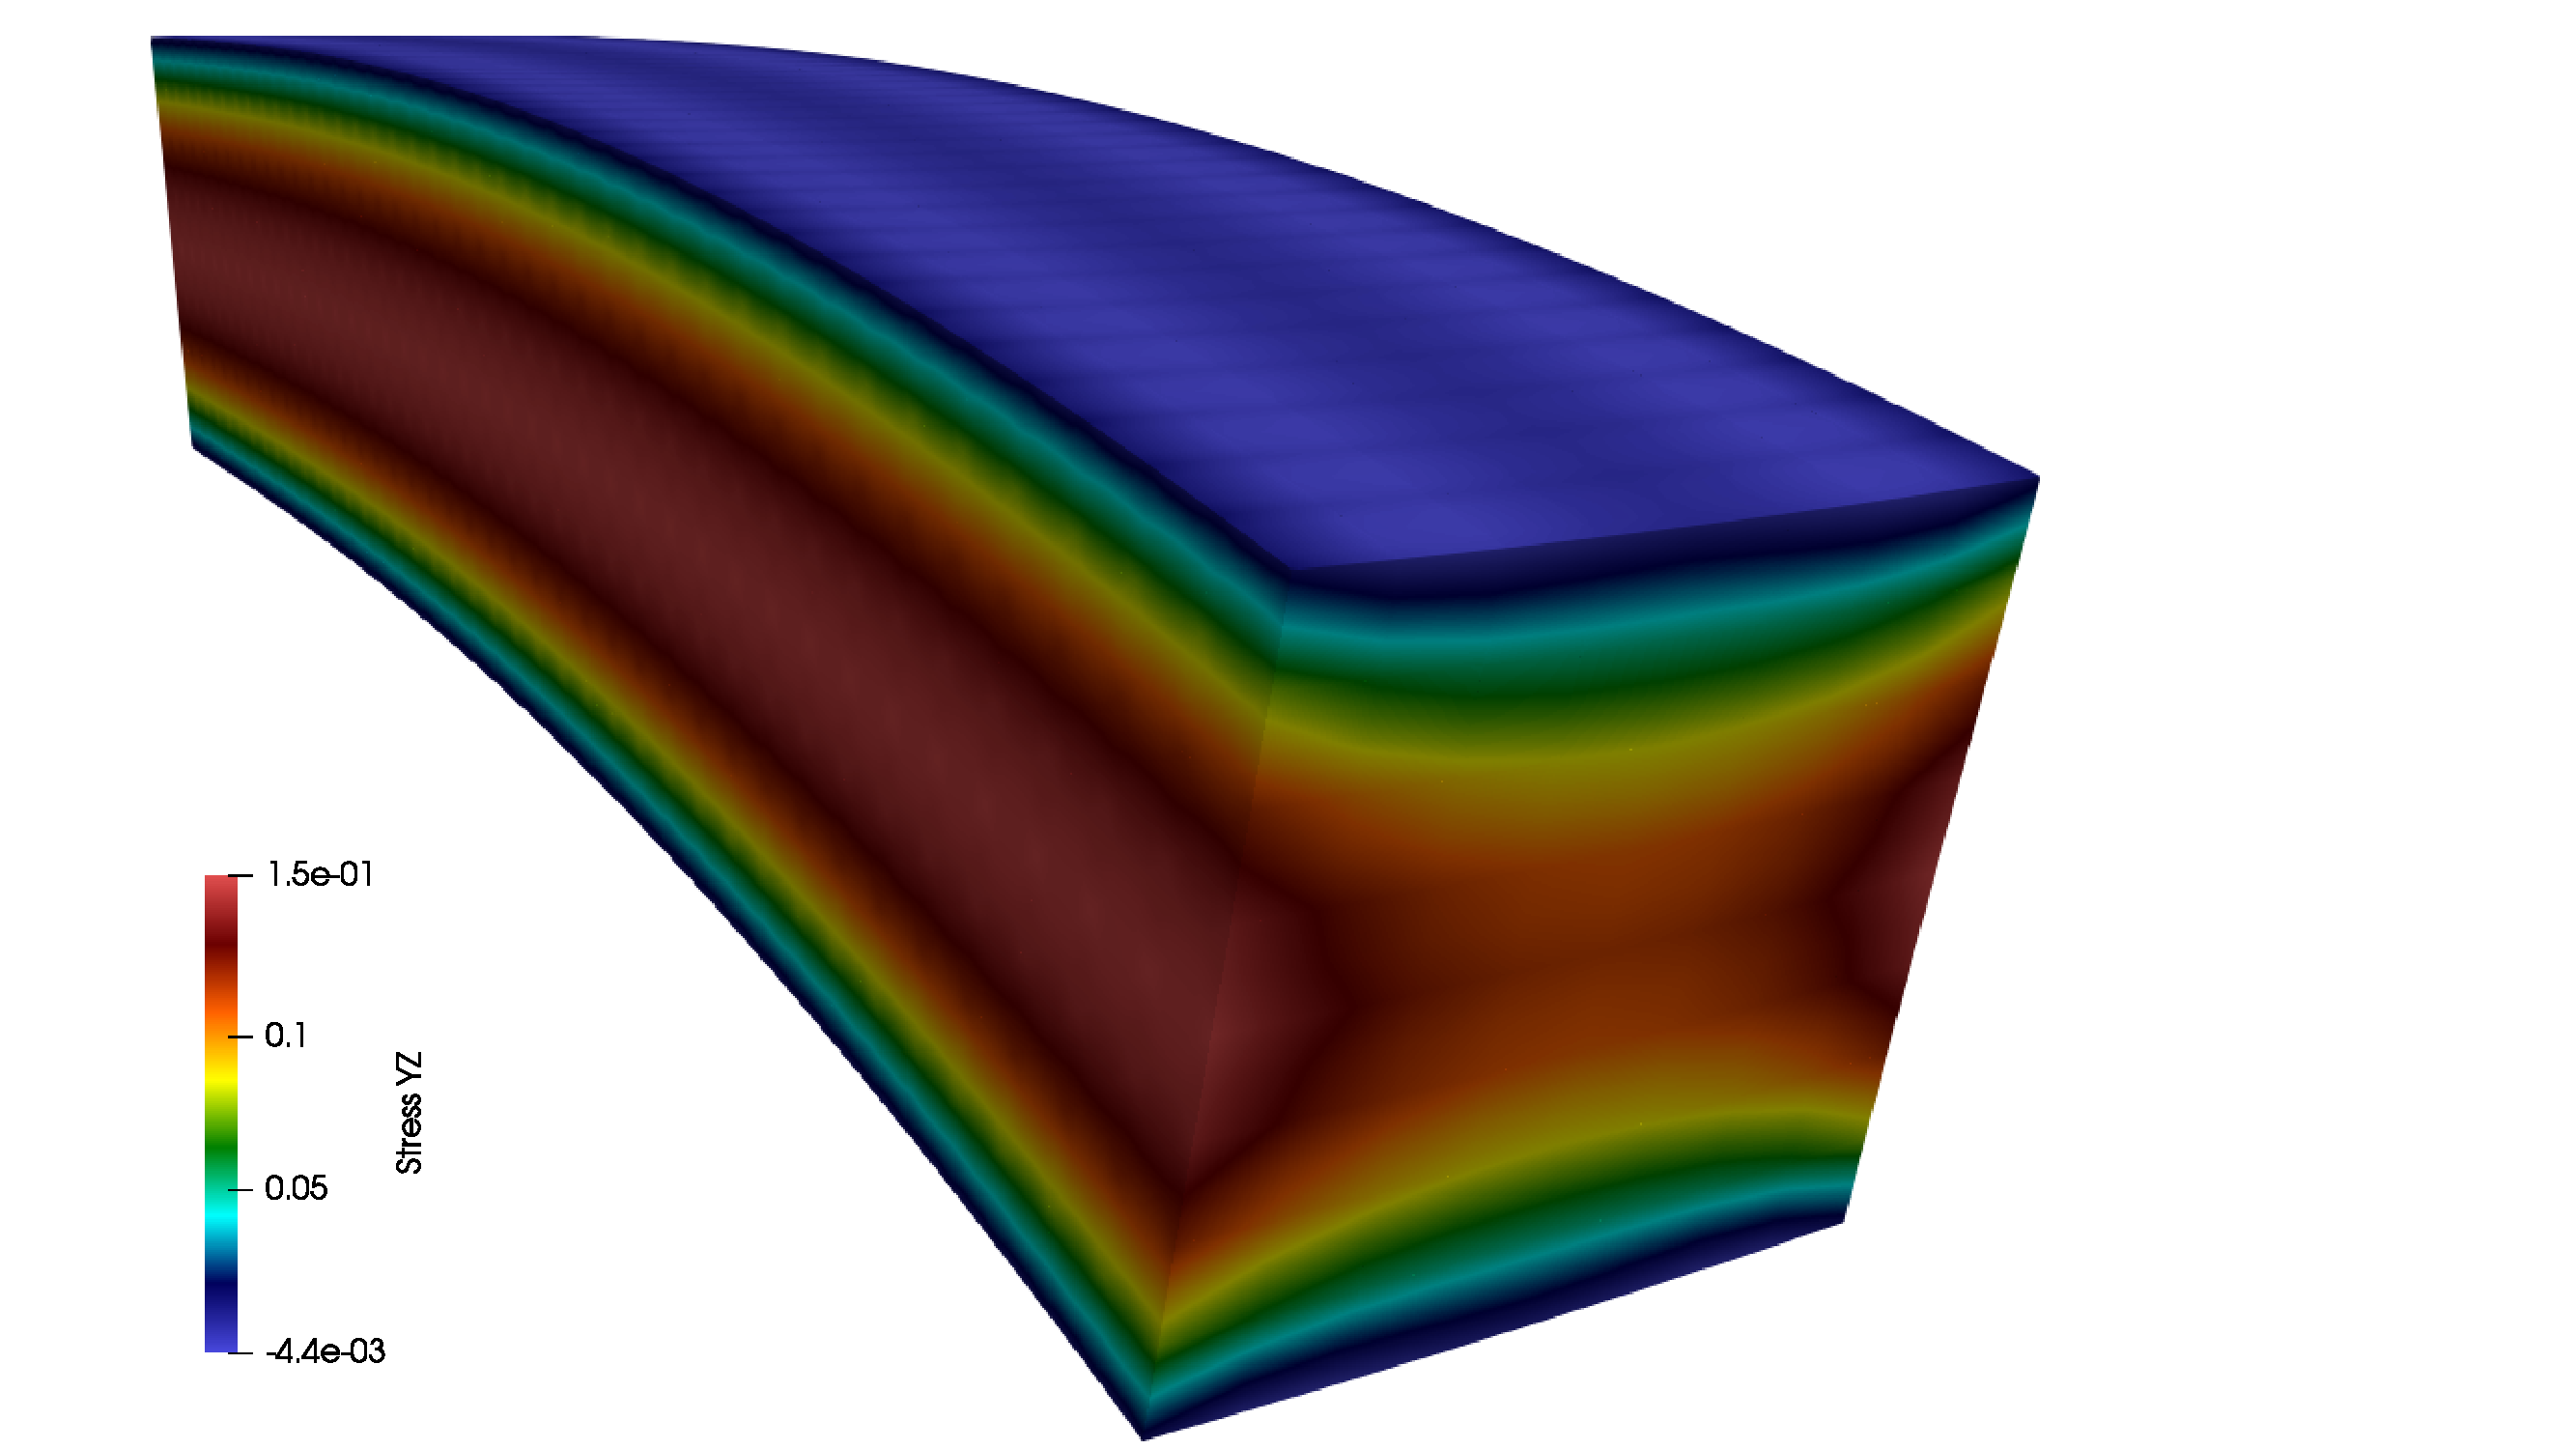
\includegraphics[trim={2.5cm 0cm 9.2cm 0cm},clip,scale=0.2]{figs/bishop-snapshot-d.pdf}}
    \caption{Cantilever beam subjected to an end shear load - snapshots for $\nu=0.3$}
    \label{fig:bishop-snapshot}
\end{figure}

\subsection{Experimental apparatus used in petroleum engineering}

The second example consists on a thin-walled structural casket that is subjected to an internal pressure load due to the filling of saturated sand. This is a real apparatus designed to run experimental analyses of the loss of injectivity of produced water in petroleum wellbores, financed by Total Energies. The hull is made of steel, with Young modulus $E=210\times 10^{3}$ MPa, poisson coefficient $\nu=0.3$, thickness $t=45.1$ mm, internal radius $R_i=344.9$ mm and length $L=1000$ mm. The internal pressure is assumed to be $p=10.34$ MPa. A real picture of the module is shown in Figure \ref{fig:casket-1}. The Von Mises stress and displacement fields are plotted in Figures \ref{fig:casket-2}-\ref{fig:casket-3}. From a qualitatively point of view, the results are in agreement with the expected physics of the problem.

\begin{figure} [!htb]
    \centering
    \subfloat[\label{fig:casket-1}]{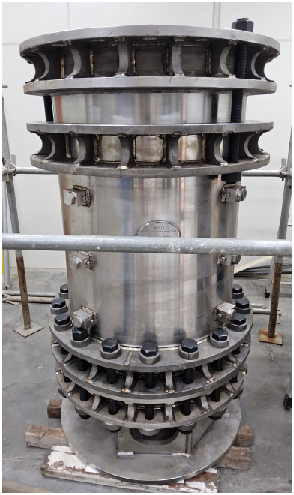
\includegraphics[scale=0.9]{figs/casket-1.pdf}} \hfill
    \subfloat[\label{fig:casket-2}]{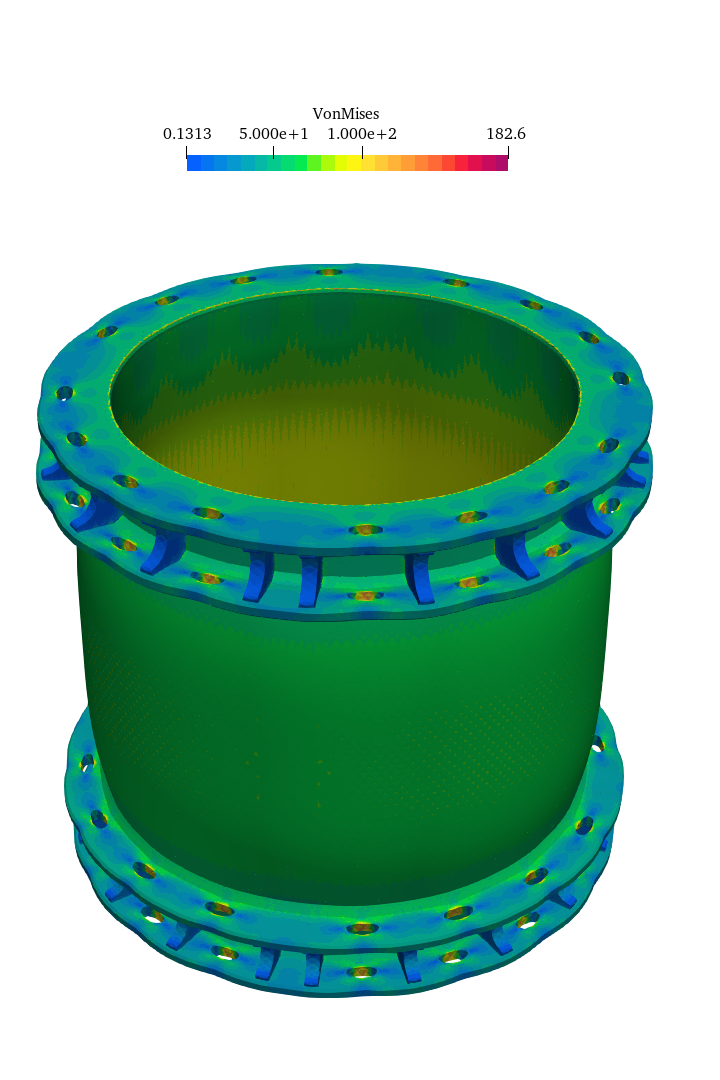
\includegraphics[scale=0.2]{figs/1m-module-vonmises.png}} \hfill
    \subfloat[\label{fig:casket-3}]{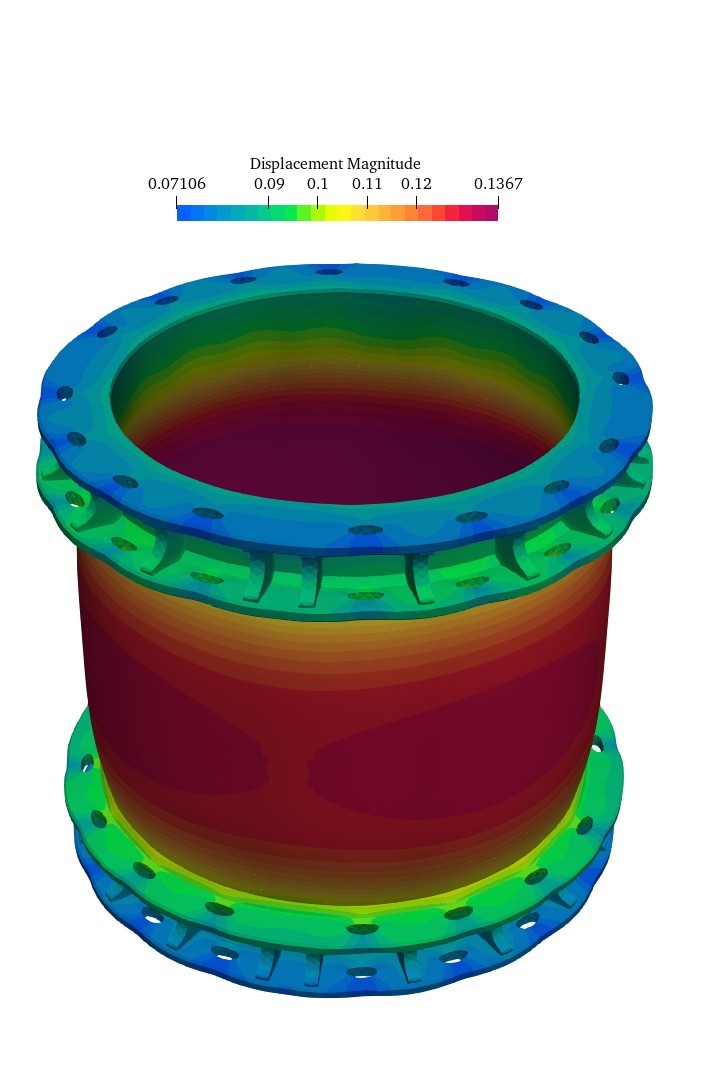
\includegraphics[scale=0.2]{figs/1m-module-disp.png}}
    \caption{Structural casket subjected to an internal pressure load - real apparatus (at left) and simulation results (Von Mises stress at center and displacement at right)}
    \label{fig:casket}
\end{figure}

\section{CONCLUSIONS}

In this work a primal hybrid formulation for tridimensional elasticity problems was developed. The approximation space composed of De Rham compatible $H(\text{div})$ functions for the normal displacements and  $L^2$ functions for the pressure leads to a locally conservative scheme. A second hybridization of the tangential stresses was applied in order to obtain positive semi definite element matrices after condensing internal degrees of freedom. The property of the resulting global system is  symmetric positive-definite matrix when analysing compressible solids and a saddle point problem with a single mean pressure per element acting as a Lagrange multiplier for incompressible materials.

The formulation was tested for a cantilever beam subjected to an end shear load and the results showed optimal convergence rates of $k+1$ for the displacement and $k$ for the remaining variables independently of the poisson coefficient. The formulation was able to capture the correct stress and displacement distributions for the compressible case and a divergence free displacement field for the incompressible case. The simulation of a real scale structural hull subjected to an internal pressure qualitatively indicates that the proposed method can be applied to real engineering problems.

\vspace{20pt}
\noindent \textbf{Acknowledgements.} We gratefully acknowledge the support of EPIC - Energy Production Innovation Center through FAPESP/Equinor (Grant 2023/06981/-5),  Total Energies Brazil through FUNCAMP (Process 76042-23) and the Brazilian National Council for Scientific and Technological Development (grants 305823/2017-5 and 309597/2021-8). We also acknowledge the support of ANP (Brazil’s National Oil, Natural Gas and Biofuels Agency).
\vspace{12pt}

\bibliographystyle{ieeetr}
\bibliography{references}

\end{document}


